\section{Field and SADAR}\label{sec:field}

\subsection{Field disposition}\label{sec:field-disposition}

\subsubsection{Choice: declared field}\label{subsec:declared-field-choice}
\paragraph{Choice.}
In this note, a field is a declared field: a retained closure structure whose memorum, regions, polychiral shell dressing, and boundaries carry returned-current orientation, duration, pressure, and closure state.

\subsubsection{Memorum}\label{subsec:field-memorum}
The field's memorum is its retained predecessor closure, present boundary, and successor horizon. A field can contain finer fields. At the next enclosing address, the entire field can be bound as one monon cycle.

\subsubsection{Region}\label{subsec:field-region}
\begin{definition}[Region]
A region is a declared retained part of a field. Regions carry current, closure, pressure, and returned-current orientation.
\end{definition}

\subsubsection{Boundary}\label{subsec:field-boundary}
\begin{definition}[Boundary]
A boundary is the retained interface of a declared region or field. Boundary accounting records current and closure across the boundary.
\end{definition}

\subsubsection{Tesseract-admissible field boundary}\label{subsec:tesseract-admissible-boundary}
When a retained field boundary is induced by the finite \(Q_4\) Hamming--1 support, write \(\partial_TF\) and use
\[
B=(\partial_TF,\omega).
\]
The formal tesseract-admissible boundary definition is given at the first \(Q_4\) / Hamming--1 derivation in \secref{subsec:q4-hamming-ternary-kernel}.

\subsubsection{Polychiral shell dressing}\label{subsec:polychiral-shell-dressing}
\begin{definition}[Polychiral shell dressing]
A polychiral shell dressing is field outer dressing. It carries Capital-Alpha/Omega return orientation, polarization imbalance, return duration, pressure, and SADAR coupling.
\end{definition}

Tritrio::Tetratrio::hexon. \appref{app:cc-basic-shared-hexon}. Dimonhexon. \appref{app:cc-standalone-enclosed-names}.

\begin{figure}[H]
\centering
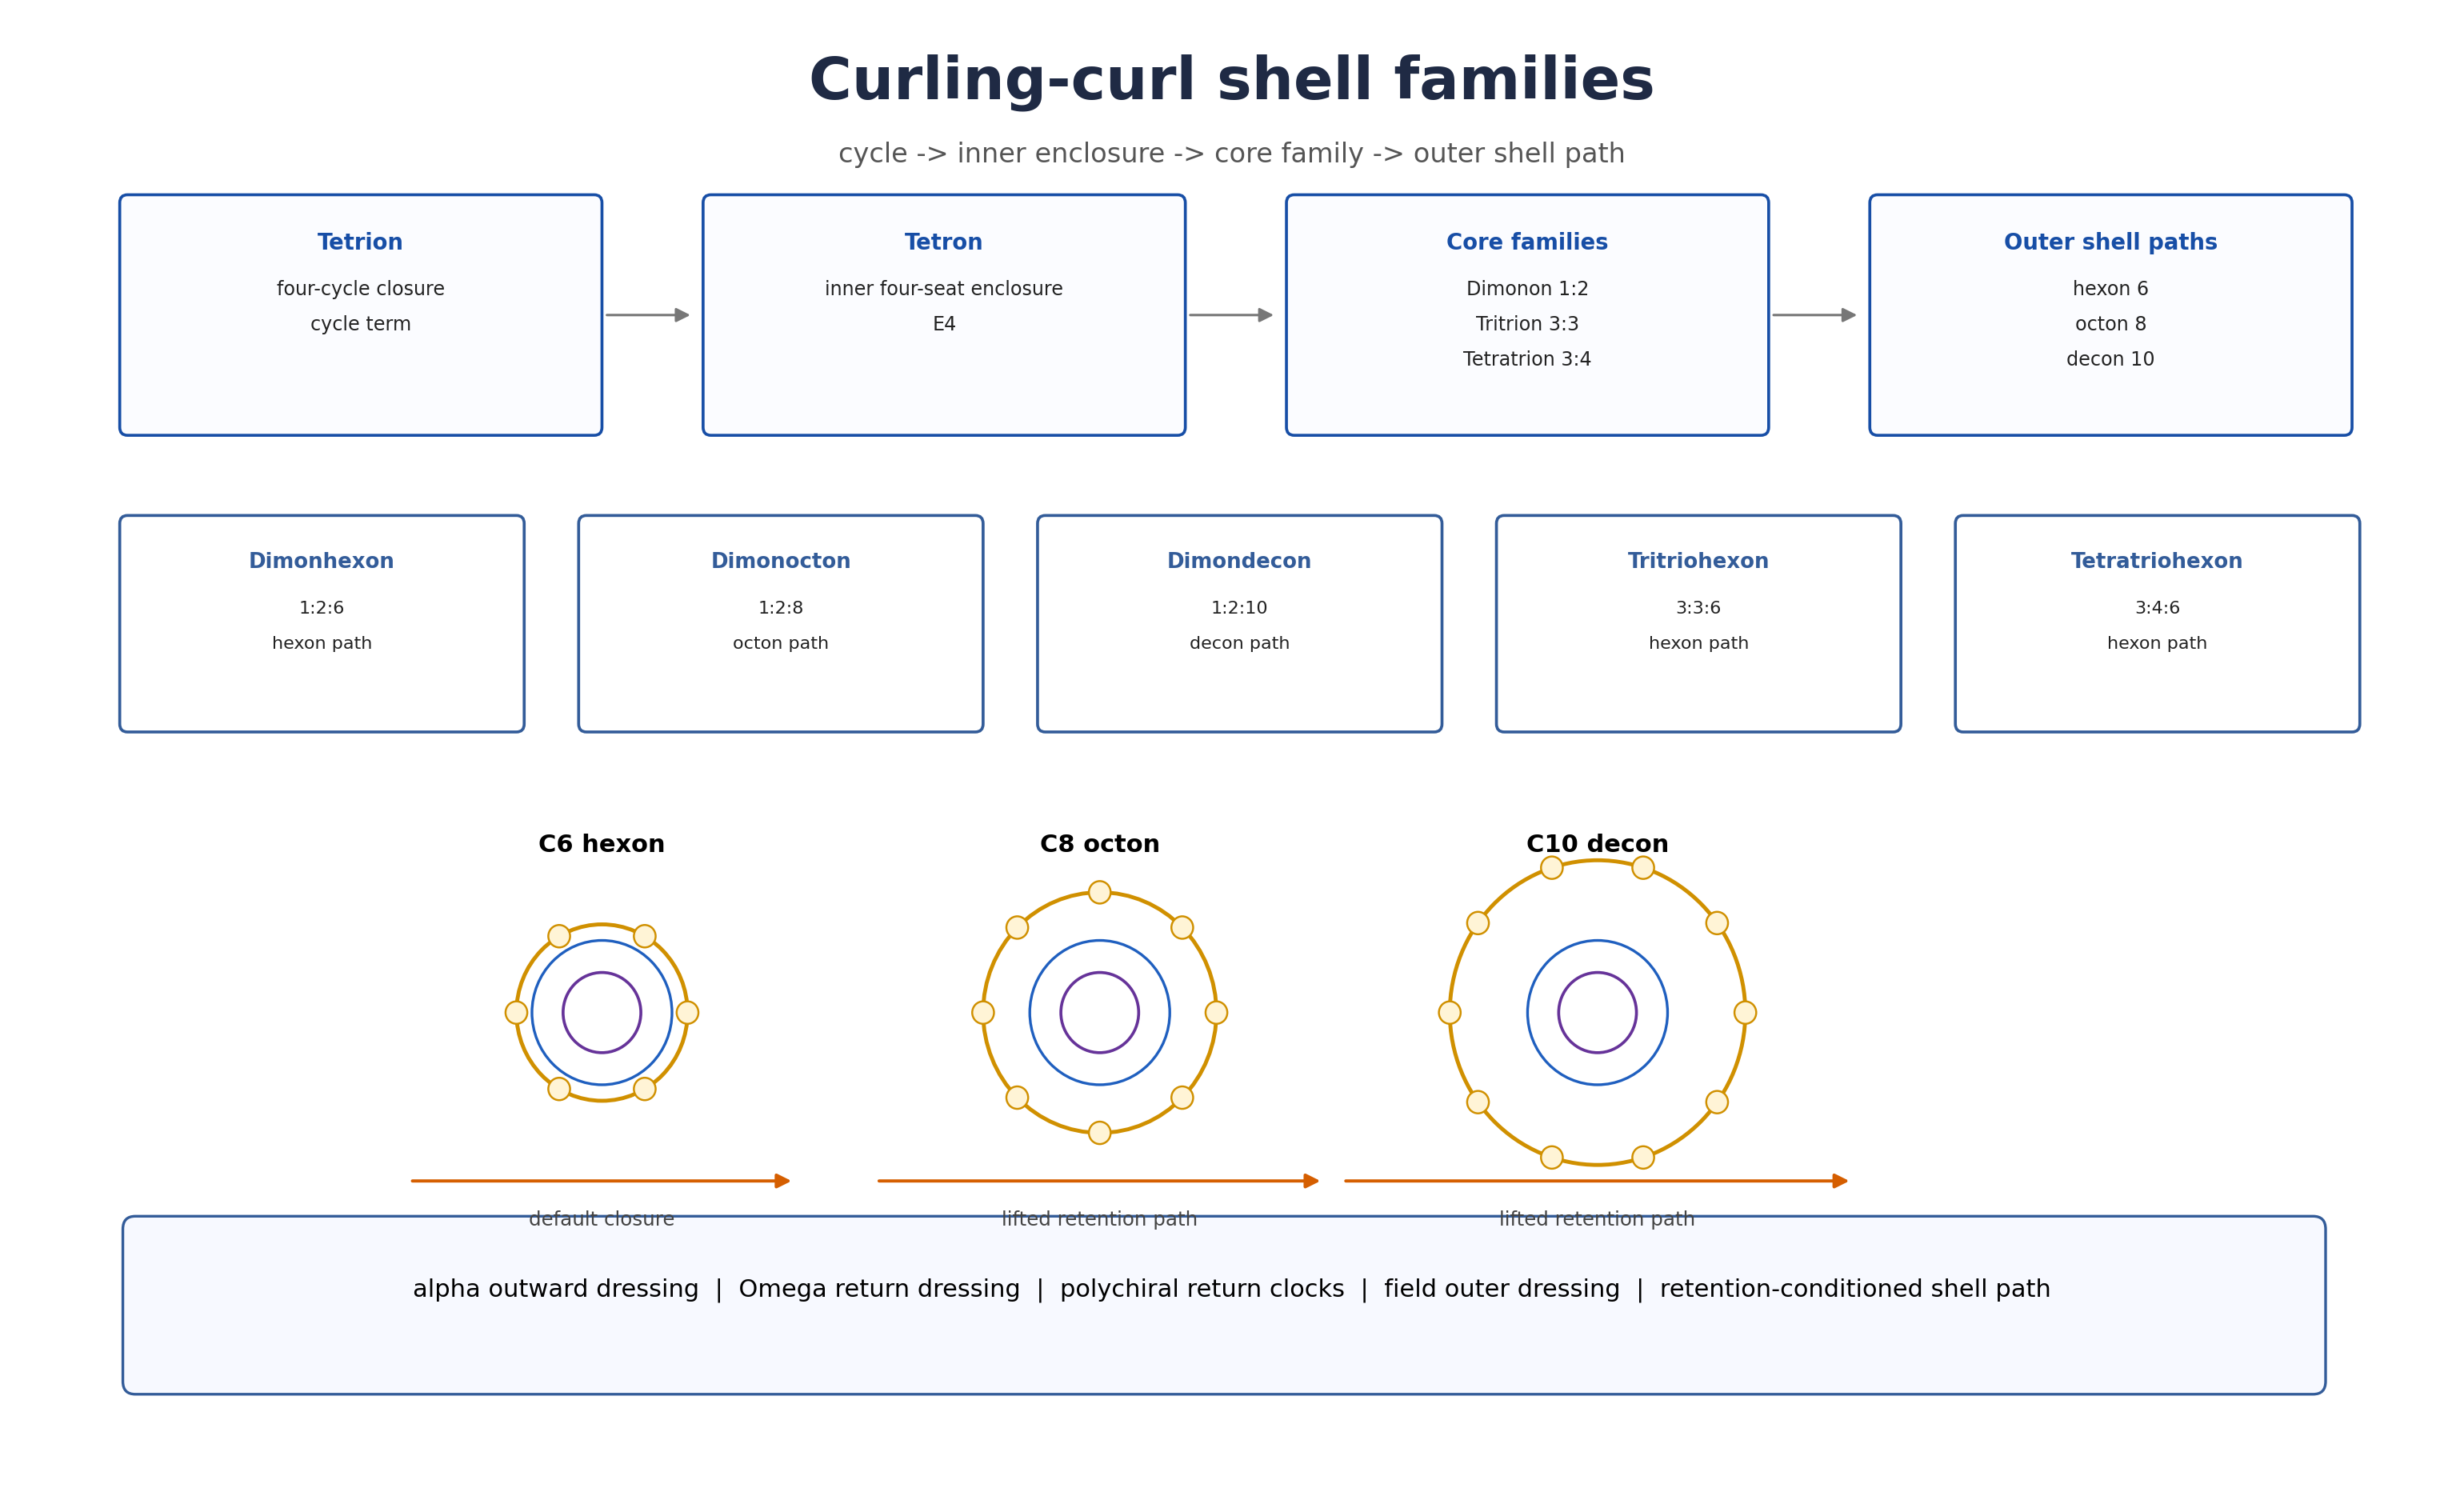
\includegraphics[width=0.96\linewidth]{figures_jpg/curling_curl_layers.png}
\caption{Curling-curl shell families.}
\label{fig:curling-curl-shell-families}
\end{figure}

\paragraph{Support-enclosure integrity.}
A tetron is \(E_4\): the default inner enclosure with four seats. Hexon, octon, and decon name outer shell paths. \appref{app:cc-support-enclosure-names}. A boundary can cut through a retained enclosure for accounting. That partial boundary is a sample of the enclosure structure. The complete enclosure identity follows the retained even-address topology.

\subsection{Field-as-monon compression}\label{subsec:field-as-monon-compression}
When a declared boundary encloses a complete retained field \(\mathcal F\), the enclosed field can be bound as one monon cycle relative to the next enclosing address:
\[
\mathrm{monon}_{\mathcal F}=\operatorname{cycle}_{\partial\mathcal F}(x\succ x=x).
\]
The internal field may contain curls, shells, temporal cycle presentations, returned-current duration, pressure, and SADAR. The enclosing boundary can still bind the whole field as one cycle.


\subsection{Cycle-valued field compression}\label{subsec:cycle-valued-field-compression}
\begin{definition}[Cycle-valued field compression]
Let \(f=\partial_T\mathcal F\) be a tesseract-admissible boundary and let \(B_f=(f,\omega_f)\). For an internal support expression \(\Sigma\), the cycle-valued field compression is
\begin{equation}
C_f[\Sigma]_{\AO}
:=
\operatorname{cycle}_{\partial_T\mathcal F}
\left[
  x\succ x=x;\ \operatorname{int}=\Sigma,\ \omega_f
\right]_{\AO}.
\label{eq:cycle-valued-field-compression}
\end{equation}
The enclosing boundary binds the retained field as one cycle. The internal support expression remains carried as cycle provenance.
\end{definition}

\subsection{Boundary accounting}\label{sec:boundary-accounting}

\subsubsection{Scope}\label{subsec:boundary-scope}
Boundary accounting records current and closure across declared field structures. A reusable regional statement has the form
\[
\mathbf a\vdash(\mathcal F,\mathcal R,\partial R,\omega),
\]
where \(\mathcal F\) is the declared field, \(\mathcal R\) is the declared retained region, \(\partial R\) is the region boundary, and \(\omega\) is the window. When the boundary is the retained tesseract-admissible shell cut, write \(\partial_T R\) or \(\partial_TF\) and use \(B=(\partial_TF,\omega)\).


\subsubsection{Returned-current duration coordinate}\label{subsec:returned-current-duration-coordinate}
The returned-current duration coordinate \(D_e(\partial F,\omega)\) is the retained duration component of a returned-current channel on the declared field boundary and window:
\begin{equation}
D_e(\partial F,\omega)=\text{duration coordinate of returned-current channel }e.
\label{eq:returned-duration}
\end{equation}
Equivalently, for an oriented channel \((i,j)\) on \(B=(\partial F,\omega)\), write \(D_{ij}(B)\).

\subsubsection{Reflection-duration coupling}\label{subsec:reflection-duration-coupling}
For a returned-current channel \((i,j)\), keep reflection-duration coupling typed as a coupled object,
\begin{equation}
\RCD_{ij}(B)=RD_B(C_{ij})\bowtie_B R^{\mathrm{asym}}_{ij}(B).
\label{eq:rcd-coupling}
\end{equation}
Its scalar duration participation is
\begin{equation}
\rho^D_{ij}(B):=\operatorname{dur}\!\left(\RCD_{ij}(B)\right).
\label{eq:rcd-duration-participation}
\end{equation}
The window-clipped duration participation is
\begin{equation}
\rho^D_{\omega,ij}(B)=\min\!\left(\rho^D_{ij}(B),|\omega|_{ij}\right).
\label{eq:window-clipped-rho}
\end{equation}
Only \(\rho^D\) is clipped. RCD is not clipped. RD is not clipped.

\subsubsection{\texorpdfstring{\(B\)-scoped flux contents}{B-scoped flux contents}}\label{subsec:b-scoped-flux-contents}
Use the AFC flux notation and scope it by the declared boundary/window
\[
B=(\partial F,\omega).
\]
The scoped flux is written \(\phi_{ij}(B)\). The declared calculation fixes the contents of \(\phi_{ij}(B)\).

For a declared path-history family \(\mathcal H_{ij}(B)\), the path-history pressure is
\begin{equation}
p^D_{ij}(B)
=
\sum_{h\in\mathcal H_{ij}(B)}
C_{3,h}\rho^D_{\omega,h}(B).
\label{eq:path-history-pressure}
\end{equation}
A compressed channel form is licensed only after the declared compression
\begin{equation}
\mathsf{Comp}_{ij}:
\{(C_{3,h},RD_h,R^{\mathrm{asym}}_h,A_h)\}_{h\in\mathcal H_{ij}(B)}
\mapsto
(C_{3,ij},\rho^D_{ij},A_{ij}).
\label{eq:path-history-compression}
\end{equation}
Under that declared compression,
\begin{equation}
p^D_{ij}(B)=C_{3,ij}\rho^D_{\omega,ij}(B)
=
C_{3,ij}\min\!\left(\rho^D_{ij}(B),|\omega|_{ij}\right).
\label{eq:b-scoped-channel-pressure}
\end{equation}
The bare-duration form is the neutral-reflection reduction:
\[
R^{\mathrm{asym}}_{ij}(B)=\mathrm{id}
\quad\Rightarrow\quad
\rho^D_{ij}(B)=D_{ij}(B).
\]
The direction term is
\begin{equation}
A_{ij}(B)=\Delta\chi^{\mathrm{lag}}_{ij}(B)i_{ij}(B).
\label{eq:b-scoped-channel-attention}
\end{equation}
Then
\begin{equation}
\phi_{ij}(B)=p^D_{ij}(B)A_{ij}(B).
\label{eq:b-scoped-flux}
\end{equation}
Equivalently,
\begin{equation}
\phi_{ij}(B)=
C_{3,ij}\rho^D_{\omega,ij}(B)
\Delta\chi^{\mathrm{lag}}_{ij}(B)i_{ij}(B).
\label{eq:b-scoped-flux-expanded}
\end{equation}
\begin{consequence}[Magnitude and direction]
The scoped flux factors as
\[
\phi_{ij}(B)=\underbrace{p^D_{ij}(B)}_{\mathrm{magnitude}}
\underbrace{A_{ij}(B)}_{\mathrm{direction}}.
\]
If \(p^D_{ij}(B)\mapsto\lambda p^D_{ij}(B)\) while \(A_{ij}(B)\) is unchanged, then \(\phi_{ij}(B)\mapsto\lambda\phi_{ij}(B)\). For the same declared channel family, \(\mathbf A_F(B)\mapsto\lambda\mathbf A_F(B)\).
\end{consequence}
The oriented channel \((i,j)\) fixes the content of \(\phi_{ij}(B)\); the reverse channel is fixed by antisymmetry:
\begin{equation}
\phi_{ji}(B)=-\phi_{ij}(B),
\qquad
\phi_{ii}(B)=0.
\label{eq:b-scoped-flux-antisymmetry}
\end{equation}
When \(i_{ij}(B)\) has components, the antisymmetry and Stokes identity are evaluated componentwise.

\begin{equation}
\operatorname{div}(i;B)=\sum_{j\in V}\phi_{ij}(B).
\label{eq:b-scoped-divergence}
\end{equation}
For \(R\subseteq V\), AFC Stokes on the declared scope \(B\) is
\begin{equation}
\sum_{i\in R}\operatorname{div}(i;B)
=
\sum_{\substack{i\in R\\j\notin R}}\phi_{ij}(B).
\label{eq:b-scoped-stokes}
\end{equation}
\begin{figure}[H]
\centering
\fbox{\begin{minipage}{0.94\linewidth}
\small
\centering
\textbf{SADAR as \(B\)-scoped AFC flux}\\[0.5em]
\begin{tabularx}{0.96\linewidth}{@{}>{\raggedright\arraybackslash}p{0.28\linewidth}>{\centering\arraybackslash}p{0.05\linewidth}>{\raggedright\arraybackslash}X@{}}
Scope & \(\to\) & \(B=(\partial F,\omega)\) \\[0.25em]
RCD & \(\to\) & \(\operatorname{RCD}_{ij}(B)=RD_B(C_{ij})\bowtie_B R^{\mathrm{asym}}_{ij}(B)\) \\[0.25em]
Scalar duration & \(\to\) & \(\rho^D_{ij}(B)=\operatorname{dur}(\operatorname{RCD}_{ij}(B))\) \\[0.25em]
Window clip & \(\to\) & \(\rho^D_{\omega,ij}(B)=\min(\rho^D_{ij}(B),|\omega|_{ij})\) \\[0.25em]
Magnitude & \(\to\) & \(p^D_{ij}(B)=C_{3,ij}\rho^D_{\omega,ij}(B)\) \\[0.25em]
Direction & \(\to\) & \(A_{ij}(B)=\Delta\chi^{\mathrm{lag}}_{ij}(B)i_{ij}(B)\) \\[0.25em]
Flux & \(\to\) & \(\phi_{ij}(B)=p^D_{ij}(B)A_{ij}(B)\) \\[0.25em]
Attention & \(\to\) & \(\mathbf A_F(B)=\sum_{(i,j)\in F(B)}\phi_{ij}(B)\) \\[0.25em]
Motion & \(\to\) & \(\operatorname{motion}_F(B)=\mathbf A_F(B)\) \\
\end{tabularx}
\end{minipage}}
\caption{SADAR as \(B\)-scoped AFC flux.}
\label{fig:sadar-b-scoped-afc-flux}
\end{figure}

\aodprovenance{\eqnref{eq:afc-stokes-used}; \eqnref{eq:afc-flux-ao-resolution}; \eqnref{eq:b-scoped-flux}; \eqnref{eq:b-scoped-stokes}.}

\subsubsection{Slice flux}\label{subsec:slice-flux}
\begin{definition}[Duon slice flux]
For a declared cut-frame \(t\), let
\[
B|_t=(\partial F,\{t\}).
\]
The duon-current slice flux is the one cut-frame crossing
\begin{equation}
\Phi^D_{\partial R}(t;B|_t)
=
\sum_{e\in\partial R(t)}
\phi_e(B|_t).
\label{eq:slice-flux}
\end{equation}
When the scope is fixed, write \(\Phi^D_{\partial R}(t)\). For raw duon-current content, \(\phi_e(B|_t)=\epsilon_e C_{3,e}\).
\end{definition}

\subsubsection{Window current}\label{subsec:window-current}
\begin{definition}[Window duon current]
The window current is the retained many-frame continuation
\begin{equation}
J^D_{\partial R}(\omega;B)
=
\sum_{t\in\omega}
\Phi^D_{\partial R}(t;B|_t).
\label{eq:window-current}
\end{equation}
When the scope is fixed, write \(J^D_{\partial R}(\omega)\).
\end{definition}
A slice flux is one declared cut-frame crossing of duon/trit current through the boundary. A window current is the retained many-frame continuation of such crossings across the declared window.

The raw capacity crossing count is
\begin{equation}
N^D_{\partial R}(\omega;B)
=
\sum_{t\in\omega}
\sum_{e\in\partial R(t)}
C_{3,e}.
\label{eq:raw-capacity-crossing-count}
\end{equation}
The magnitude current is
\begin{equation}
J^D_{\mathrm{mag}}(\omega;B)
=
\sum_{t\in\omega}
\sum_{e\in\partial R(t)}
p^D_e(B|_t).
\label{eq:magnitude-current}
\end{equation}
When the declared boundary/window partitions current status, require
\begin{equation}
J^D_{\mathrm{mag}}
=
J^D_{\mathrm{in}}+J^D_{\mathrm{out}}+J^D_{\mathrm{pending}}.
\label{eq:current-magnitude-split}
\end{equation}

\subsubsection{Moving boundary}\label{subsec:moving-boundary}
For a moving retained boundary, the window may record crossing, sweep, and shedding terms as
\begin{equation}
\Phi^D_{\partial R,\mathrm{mov}}(t)
=
\Phi^D_{\mathrm{cross}}(t)
-
\Phi^D_{\mathrm{sweep}}(t)
+
\Phi^D_{\mathrm{shedding}}(t).
\label{eq:moving-boundary}
\end{equation}
Here crossing is duon current crossing the retained boundary, sweep is support swept by boundary motion, and shedding is disturbance that breaks from the retained boundary.

\subsubsection{Regional boundary template}\label{subsec:regional-boundary-template}
The same boundary/current form applies across familiar region choices. Declare a region, declare \(\partial R\), and account for current crossing, returning, and remaining pending.

\begin{figure}[H]
\centering
\fbox{\begin{minipage}{0.94\linewidth}
\small
\centering
\textbf{Duon-current boundary accounting}\\[0.5em]
\begin{tabularx}{0.96\linewidth}{@{}XXXX@{}}
\textbf{Internal retained} & \textbf{Exoshedding} & \textbf{Reflected return} & \textbf{Pending return}\\
recurring core & crosses \(\partial R\) & returns through shell & remains over \(\omega\)\\
scalar burden & shell crossing & next emission & duration overlap\\
\end{tabularx}\\[0.6em]
\begin{minipage}{0.92\linewidth}
\centering
\(\Phi^D_{\partial R}(t;B|_t)=\sum_{e\in\partial R(t)}\phi_e(B|_t)\)\\[0.25em]
\(J^D_{\partial R}(\omega;B)=\sum_{t\in\omega}\Phi^D_{\partial R}(t;B|_t)\)
\end{minipage}
\end{minipage}}
\caption{Duon-current boundary accounting.}
\label{fig:v39-duon-current-boundary-accounting}
\end{figure}

\aodprovenance{\eqnref{eq:duon-current},
\eqnref{eq:slice-flux},
\eqnref{eq:window-current},
\eqnref{eq:moving-boundary}.}

\subsection{Field count}\label{sec:field-count-sadar-scope}

\subsubsection{Scope}\label{subsec:field-count-fixed-scope}
Fix a boundary/window scope
\[
\mathcal B=(\partial F,\omega).
\]
All quantities in this subsection are evaluated with respect to \(\mathcal B\).

\subsubsection{Retained field family}\label{subsec:retained-field-family}
Let
\[
\mathcal F_{\mathcal B}=\{F_1,\ldots,F_{n_F}\}
\]
be the retained field family, and define
\begin{equation}
n_F(\mathcal B):=|\mathcal F_{\mathcal B}|.
\label{eq:field-count}
\end{equation}
Here \(n_F\) is retained field count, \(T\) is path/account duration or tick count, \(m\) is enclosure order in \(\mathsf C_{2m}\), and \(p\) is rotor or cycle completion period.

\subsubsection{Returned-current channels}\label{subsec:returned-current-channels}
For \(F_i,F_j\in\mathcal F_{\mathcal B}\), write
\[
\ADAR_{i\leftarrow j}
\]
for the returned-current channel from \(F_j\) into \(F_i\). The diagonal terms are self-return terms; off-diagonal terms are cross-return terms. A retained field family may carry field-ring returned-current relations when \(E_{\mathrm{return}}\) is declared on the fixed boundary/window.

\subsubsection{Field-count term}\label{subsec:field-count-term}
The field-count contribution entering the SADAR calculation is
\begin{equation}
\mathcal O_{\partial F}(\mathcal B)=n_F(\mathcal B)\log n_F(\mathcal B),
\label{eq:field-count-term}
\end{equation}
with the logarithm base fixed by the declared calculation. The monon case \(n_F=1\) is the unit retained-field anchor. Coupled-field counting begins at \(n_F=2\).

\subsubsection{Disoma declaration}\label{subsec:disoma-declaration}
For a two-field declared scope, fix
\[
B_{12}=(\partial F_{12},\omega_{12}),
\qquad
\mathcal F_{B_{12}}=\{F_1,F_2\}.
\]
Thus
\[
n_F(B_{12})=2,
\qquad
\mathcal O_{\partial F}(B_{12})=2\log 2.
\]

\paragraph{Calculation split.}
Field-count scaling and shell/enclosure routing are connected by the declared boundary/window, but they are separate calculations:
\[
B\to \mathcal F_{B}\to n_F(B)\to \ADAR_{i\leftarrow j}\to \mathcal O_{\partial F}(B)\to \SADAR.
\]
Shell/enclosure routing fixes
\[
\begin{aligned}
\mathcal C_{2m}
&\to X_{\mathrm{shedding}}
\to \mathrm{SheddicPath}(X_{\mathrm{shedding}}),\\
\mathrm{SheddicPath}
&\to
\{\text{rebalancing},\ \text{exoshedding},\ \text{endoshedding},\ \text{redirected support routing}\}.
\end{aligned}
\]

\begin{figure}[H]
\centering
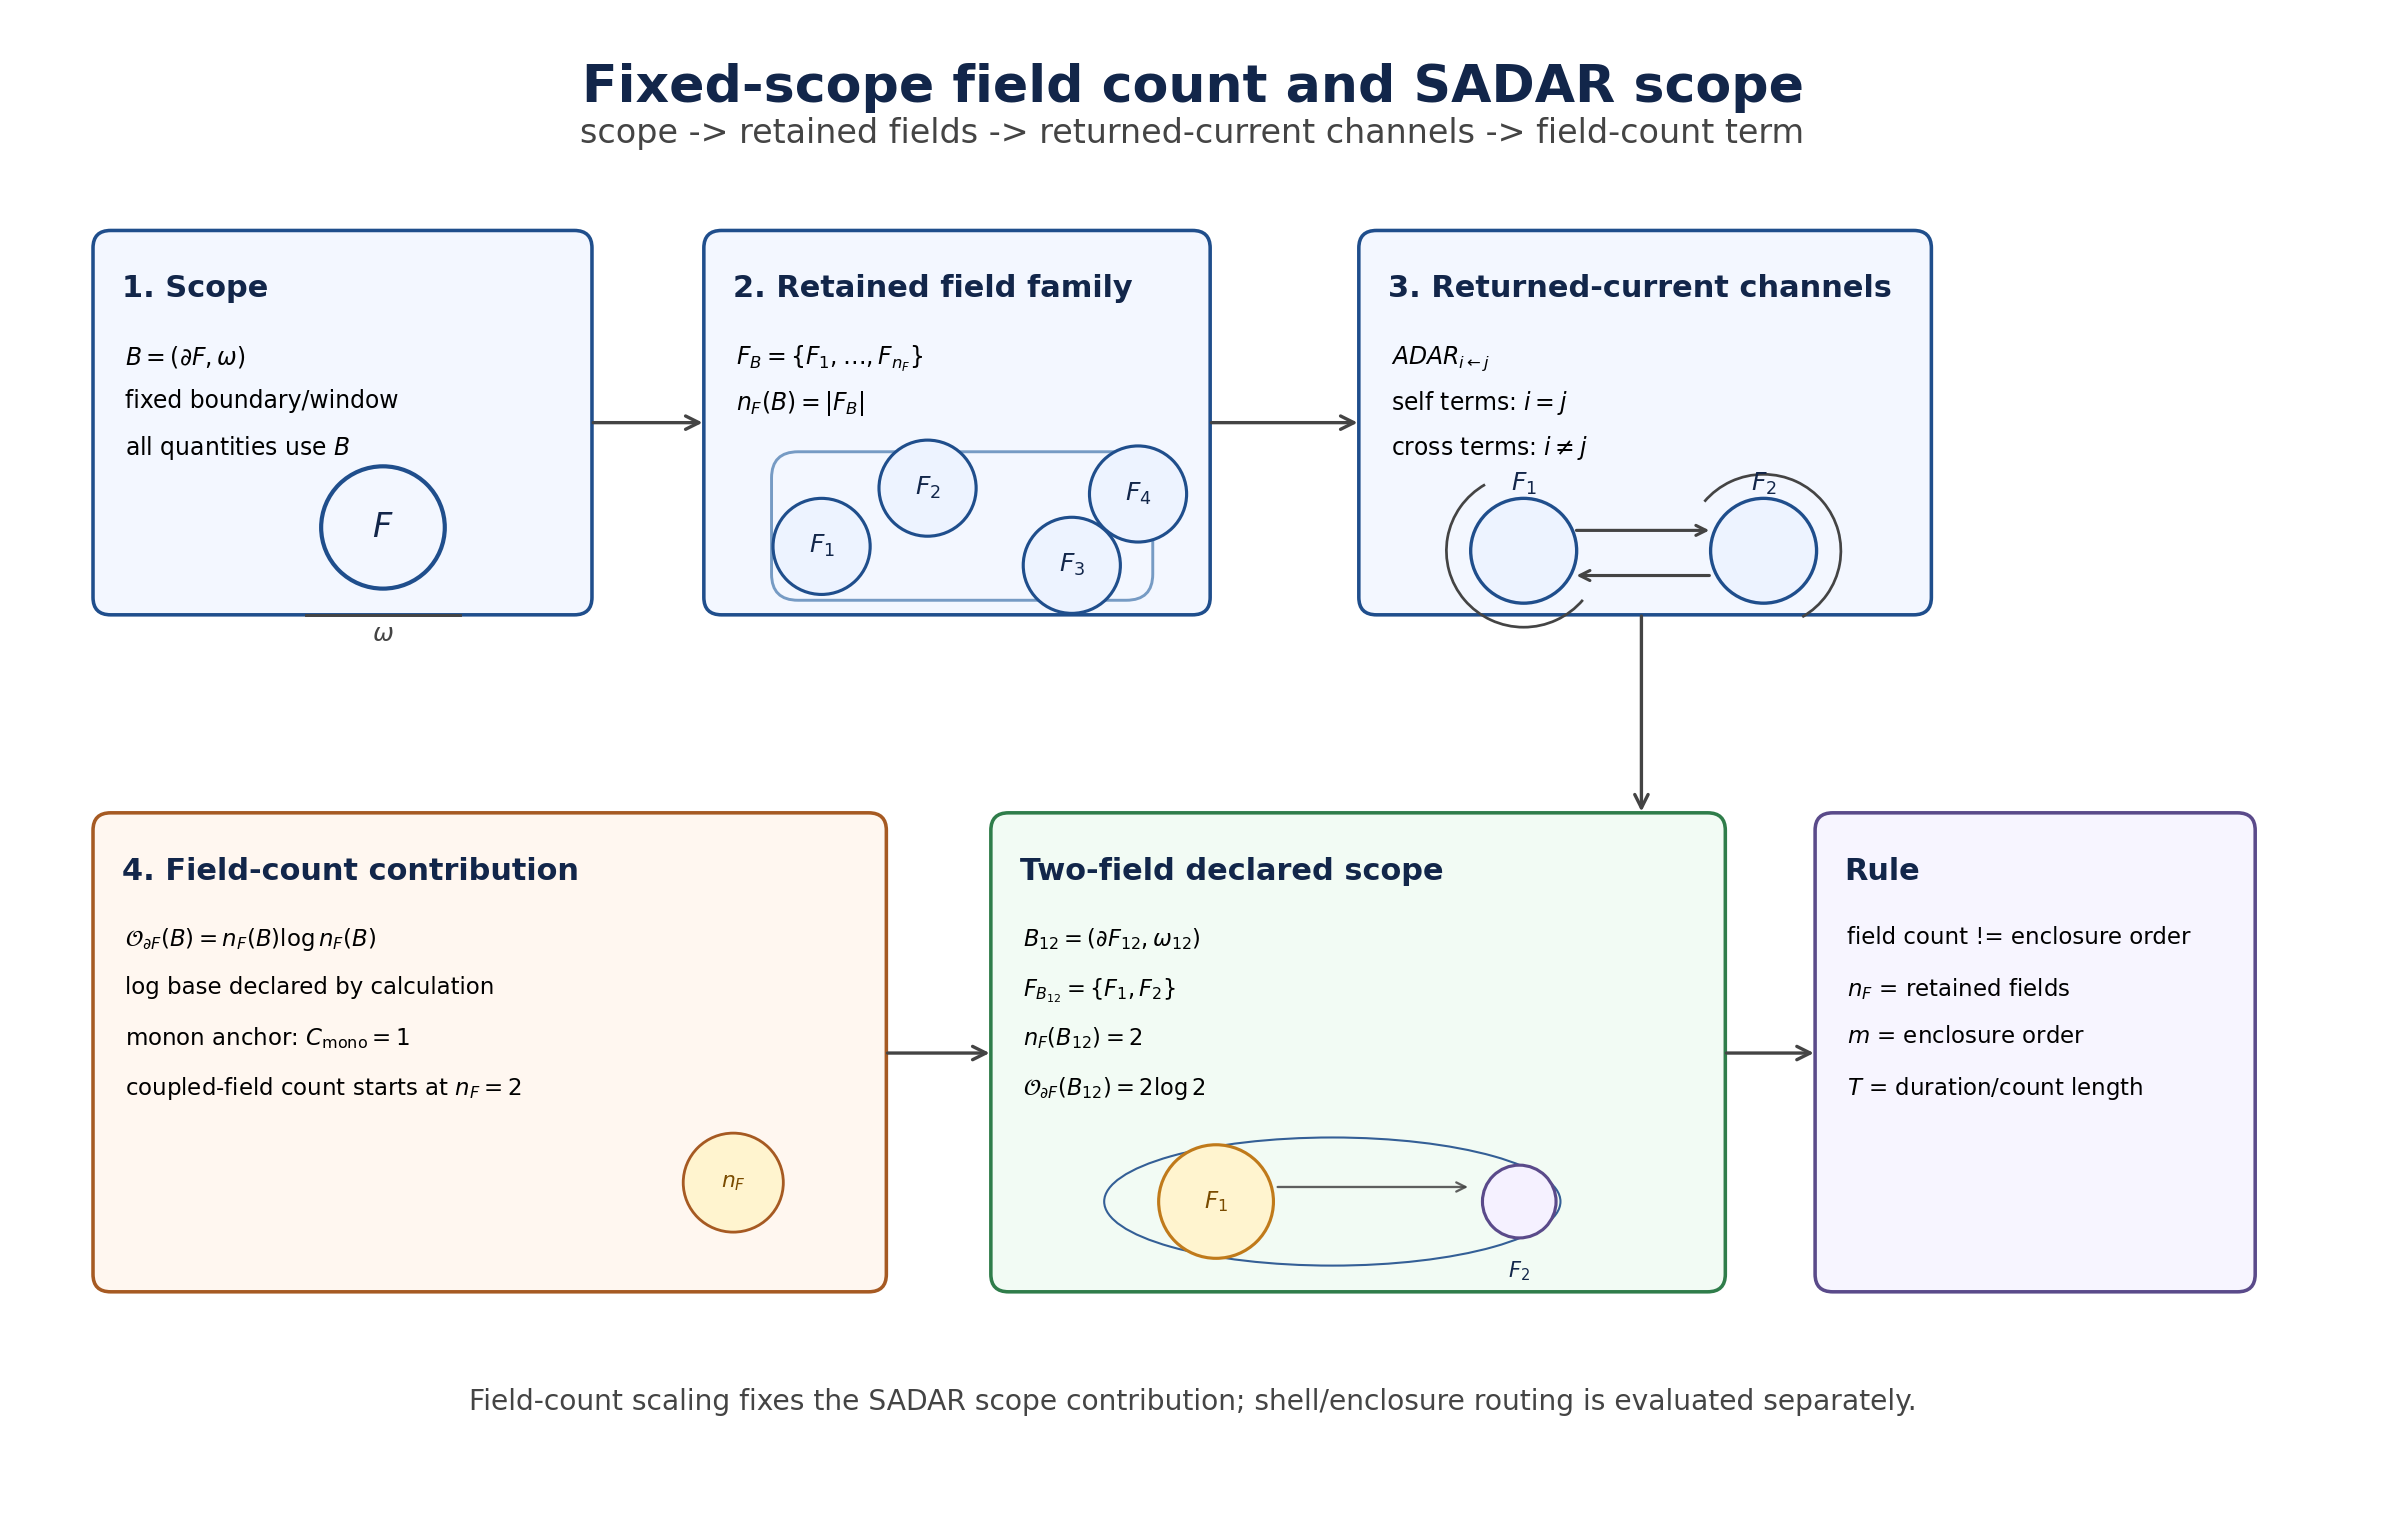
\includegraphics[width=0.96\linewidth]{figures_jpg/fixed_scope_field_count.png}
\caption{Fixed-scope field count and SADAR scope.}
\label{fig:field-count}
\end{figure}

\aodprovenance{\eqnref{eq:field-count},
\eqnref{eq:field-count-term},
\eqnref{eq:sadar-field}.}

\subsection{Duonic pressure}\label{sec:duonic-pressure-inertia}

\subsubsection{Scalar burden}\label{subsec:duonic-pressure-scalar-burden}
\begin{definition}[Channel pressure]
For a returned duon-current channel \(e\) on \(B=(\partial F,\omega)\), channel pressure uses the window-clipped duration participation:
\[
p^D_e(B)=C_{3,e}\rho^D_{\omega,e}(B).
\]
Here \(\rho^D_\omega\) is the window-clipped duration participation. It is distinct from \(TTL_{\mathcal C}\), the seat-compatible retention duration of a support enclosure or sheddic path.
\end{definition}
\begin{definition}[Duonic pressure]
The scalar pressure of a field is
\begin{equation}
P^D_F(B)=
\sum_{e\in F(B)}p^D_e(B).
\label{eq:duonic-pressure}
\end{equation}
It records the retained/clipped duon/trit burden carried on the declared boundary/window; pending overhang is recorded separately by \(Q^D\).
\end{definition}

\subsubsection{Pressure weighting}\label{subsec:duonic-pressure-weighting}
When \(P^D_F(B)>0\), a normalized orientation \(\theta_F^{(q)}\) may be weighted by scalar pressure to provide scalar factors later used in \(\mathbf A_F(B)\) in \secref{sec:field:sadar}.

\subsubsection{Inertial burden}\label{subsec:inertial-burden}
Duonic pressure resists change of attention orientation. A perturbing duon current changes normalized orientation in inverse proportion to retained pressure:
\[
\Delta\theta_F^{(q)}=
\frac{\Delta J_{\mathrm{duon}}^{(q)}}{P^D_F(B)}.
\]

\aodprovenance{\eqnref{eq:entropic-duon-current},
\eqnref{eq:duonic-pressure}.}



\subsection{SADAR value operator}\label{subsec:sadar-operator}
\begin{definition}[SADAR operator]
Write \(\SADARop_B\) for Symmetry Attention Duration Asymmetric Reflection (SADAR) on the declared boundary/window \(B\). For a retained cycle \(C\),
\begin{equation}
\SADARop_B(C)
=
\phi_{C,\AO}(B)
=
p^D_{C,\AO}(B)A_{C,\AO}(B).
\label{eq:sadar-operator-cycle}
\end{equation}
Expanded,
\begin{equation}
\SADARop_B(C)
=
C_{3,C}\rho^D_{\omega,C}(B)\,\Delta\chi_C^{\mathrm{lag}}(B)i_C(B).
\label{eq:sadar-operator-expanded}
\end{equation}
For two SADAR-coupled beats \(C_u,C_v\),
\begin{equation}
\SADARop_B(C_u,C_v)
=
\phi^{\mathrm{beat}}_{uv,\AO}(B)
=
p^D_{uv,\AO}(B)A_{uv,\AO}(B).
\label{eq:sadar-operator-beat-coupling}
\end{equation}
\end{definition}
If \(\bar e\) is the reversed oriented boundary element of \(e\), then
\begin{equation}
\SADARop_B(C_{\bar e})=-\SADARop_B(C_e).
\label{eq:sadar-orientation-antisymmetry}
\end{equation}


\subsection{SADAR}\label{sec:field:sadar}

\subsubsection{ADAR channel}\label{subsec:adar-channel}
\begin{definition}[ADAR]
ADAR is one local returned-current channel:
\begin{equation}
\ADAR_{ij}(B)=(A_{ij}(B),D_{ij}(B),R^{\mathrm{asym}}_{ij}(B)).
\label{eq:adar-channel}
\end{equation}
Here \(A_{ij}(B)\) is returned-current attention orientation, \(D_{ij}(B)\) is returned-current duration, and \(R_{ij}^{\mathrm{asym}}(B)\) is asymmetric reflection on the declared boundary/window. The attention term is \(A_{ij}(B)=\Delta\chi^{\mathrm{lag}}_{ij}(B)i_{ij}(B)\).
\end{definition}

\subsubsection{SADAR balance}\label{subsec:sadar-balance}
\begin{definition}[SADAR]
SADAR is Symmetric Attention--Duration--Asymmetric Reflection: the field's symmetry-chasing returned-current dynamic on a declared boundary/window. For \(B=(\partial F,\omega)\),
\begin{equation}
\SADAR_F(B)=
\big(\ADAR_{ij}(B)\big)_{(i,j)\in F(B)}.
\label{eq:sadar-field}
\end{equation}
\end{definition}
The indexed family denotes the declared returned-current channels on \(B\), taken with their boundary incidence, phase relation, and pressure contribution. Field symmetry is the relative SADAR balance of returned duon current on \(B\). The field chases this balance through attention, duration, asymmetric reflection, phase bias, reseating, and shedding.

\subsubsection{SADAR attention vector}\label{subsec:sadar-attention-vector}
\begin{definition}[SADAR attention vector]
The SADAR attention vector is the boundary/window-specific codification of SADAR dynamics. It records pressure-weighted relational motion of returned duon current on the declared boundary/window:
\begin{equation}
\mathbf A_F(B)=
\sum_{(i,j)\in F(B)}
\phi_{ij}(B).
\label{eq:sadar-attention-vector}
\end{equation}
Equivalently,
\begin{equation}
\mathbf A_F(B)=
\sum_{(i,j)\in F(B)}
C_{3,ij}\rho^D_{\omega,ij}(B)
\Delta\chi^{\mathrm{lag}}_{ij}(B)i_{ij}(B).
\label{eq:sadar-attention-vector-expanded}
\end{equation}
\end{definition}
The scoped AFC flux \(\phi_{ij}(B)\) carries SADAR contents. The product \(C_{3,ij}\rho^D_{\omega,ij}(B)\) is the duonic-pressure contribution on \(B\); \(\Delta\chi^{\mathrm{lag}}_{ij}(B)i_{ij}(B)\) is the phase-bias / boundary-orientation contribution.

\subsubsection{Phase bias, push/pull, and motion}\label{subsec:phase-bias-motion}
Phase bias is the signed lead--lag imbalance of returned-current channels. Push and pull are signed phase-biased components of the same SADAR attention vector.
\begin{definition}[Motion]
Motion is phase-biased SADAR balance on \(B\):
\begin{equation}
\operatorname{motion}_F(B)=\mathbf A_F(B).
\label{eq:motion-sadar-attention}
\end{equation}
\end{definition}
\paragraph{Statement: incident return shift.}
If \(\mathbf A_F(B)=0\) and an unmatched incident returned duon \(e\) contributes
\[
\phi_e(B)=p^D_e(B)A_e(B),
\]
then
\begin{equation}
\mathbf A_{F+e}(B)=\phi_e(B).
\label{eq:incident-return-shift}
\end{equation}
If a matching return \(\bar e\) is declared and \(\phi_{\bar e}(B)=-\phi_e(B)\), then
\begin{equation}
\mathbf A_{F+e+\bar e}(B)=0.
\label{eq:matched-return-cancellation}
\end{equation}

\paragraph{Statement: short window and high incident current.}
If \(|\omega|_h<\rho^D_h(B)\), then \(\rho^D_{\omega,h}(B)=|\omega|_h\) and \(Q^D_h(B)>0\). For a short window,
\[
p^D_h(B)=C_{3,h}|\omega|_h.
\]
Many incident histories or large \(C_{3,h}\) can still shift the SADAR attention vector when
\[
\sum_h p^D_h(B)A_h(B)\ne0.
\]

The channel-level rate form is
\[
\Delta\phi_{ij}=p^D_{ij}\Delta A_{ij}
\]
when retained pressure is fixed across the compared restrictions. Pending overhang separates from clipped pressure:
\begin{equation}
Q^{D,\mathrm{dur}}_{ij}(B)=\max\!\left(0,\rho^D_{ij}(B)-|\omega|_{ij}\right),
\label{eq:duration-overhang}
\end{equation}
\begin{equation}
Q^D_{ij}(B)=C_{3,ij}Q^{D,\mathrm{dur}}_{ij}(B).
\label{eq:burden-overhang}
\end{equation}
A falling field may remain internally balanced relative to its own boundary/window while its SADAR attention vector is phase-biased relative to another declared boundary.

\subsubsection{Self-return and cross-return}\label{subsec:self-cross-return}
A single declared field carries self-return symmetry:
\[
\ADAR_{i\leftarrow i}=\text{self-return channel}.
\]
When another field is included in the same accounting scope, cross-return channels are added:
\[
\ADAR_{i\leftarrow j}=\text{cross-return channel},\qquad i\ne j.
\]
Self-return and cross-return are channel forms inside the same SADAR balance. A field ring gate is a finite cross-return fixture with declared boundary gates, returned-current relations, and output bins.

\subsubsection{Boundary-relative simultaneity}\label{subsec:boundary-relative-simultaneity}
Boundary-relative simultaneity names the coexistence of component-field and enclosing-field SADAR balances. Component fields and enclosing fields may each carry their own SADAR attention vector because each vector is scoped by its declared boundary/window. For the enclosing two-field scope, write
\[
\mathcal{B}_{12}=(\partial F_{12},\omega_{12}).
\]
Then
\[
\mathbf A_{F_1}(B_1),
\qquad
\mathbf A_{F_2}(B_2),
\qquad
\mathbf A_{F_1\parallel F_2}(\mathcal{B}_{12}).
\]
For three fields, write
\[
\mathcal{B}_{123}=(\partial F_{123},\omega_{123}),
\]
and
\[
\mathbf A_{F_1}(B_1),\quad
\mathbf A_{F_2}(B_2),\quad
\mathbf A_{F_3}(B_3),\quad
\mathbf A_{F_{12}}(\mathcal{B}_{12}),\quad
\mathbf A_{F_{123}}(\mathcal{B}_{123}).
\]

\begin{figure}[H]
\centering
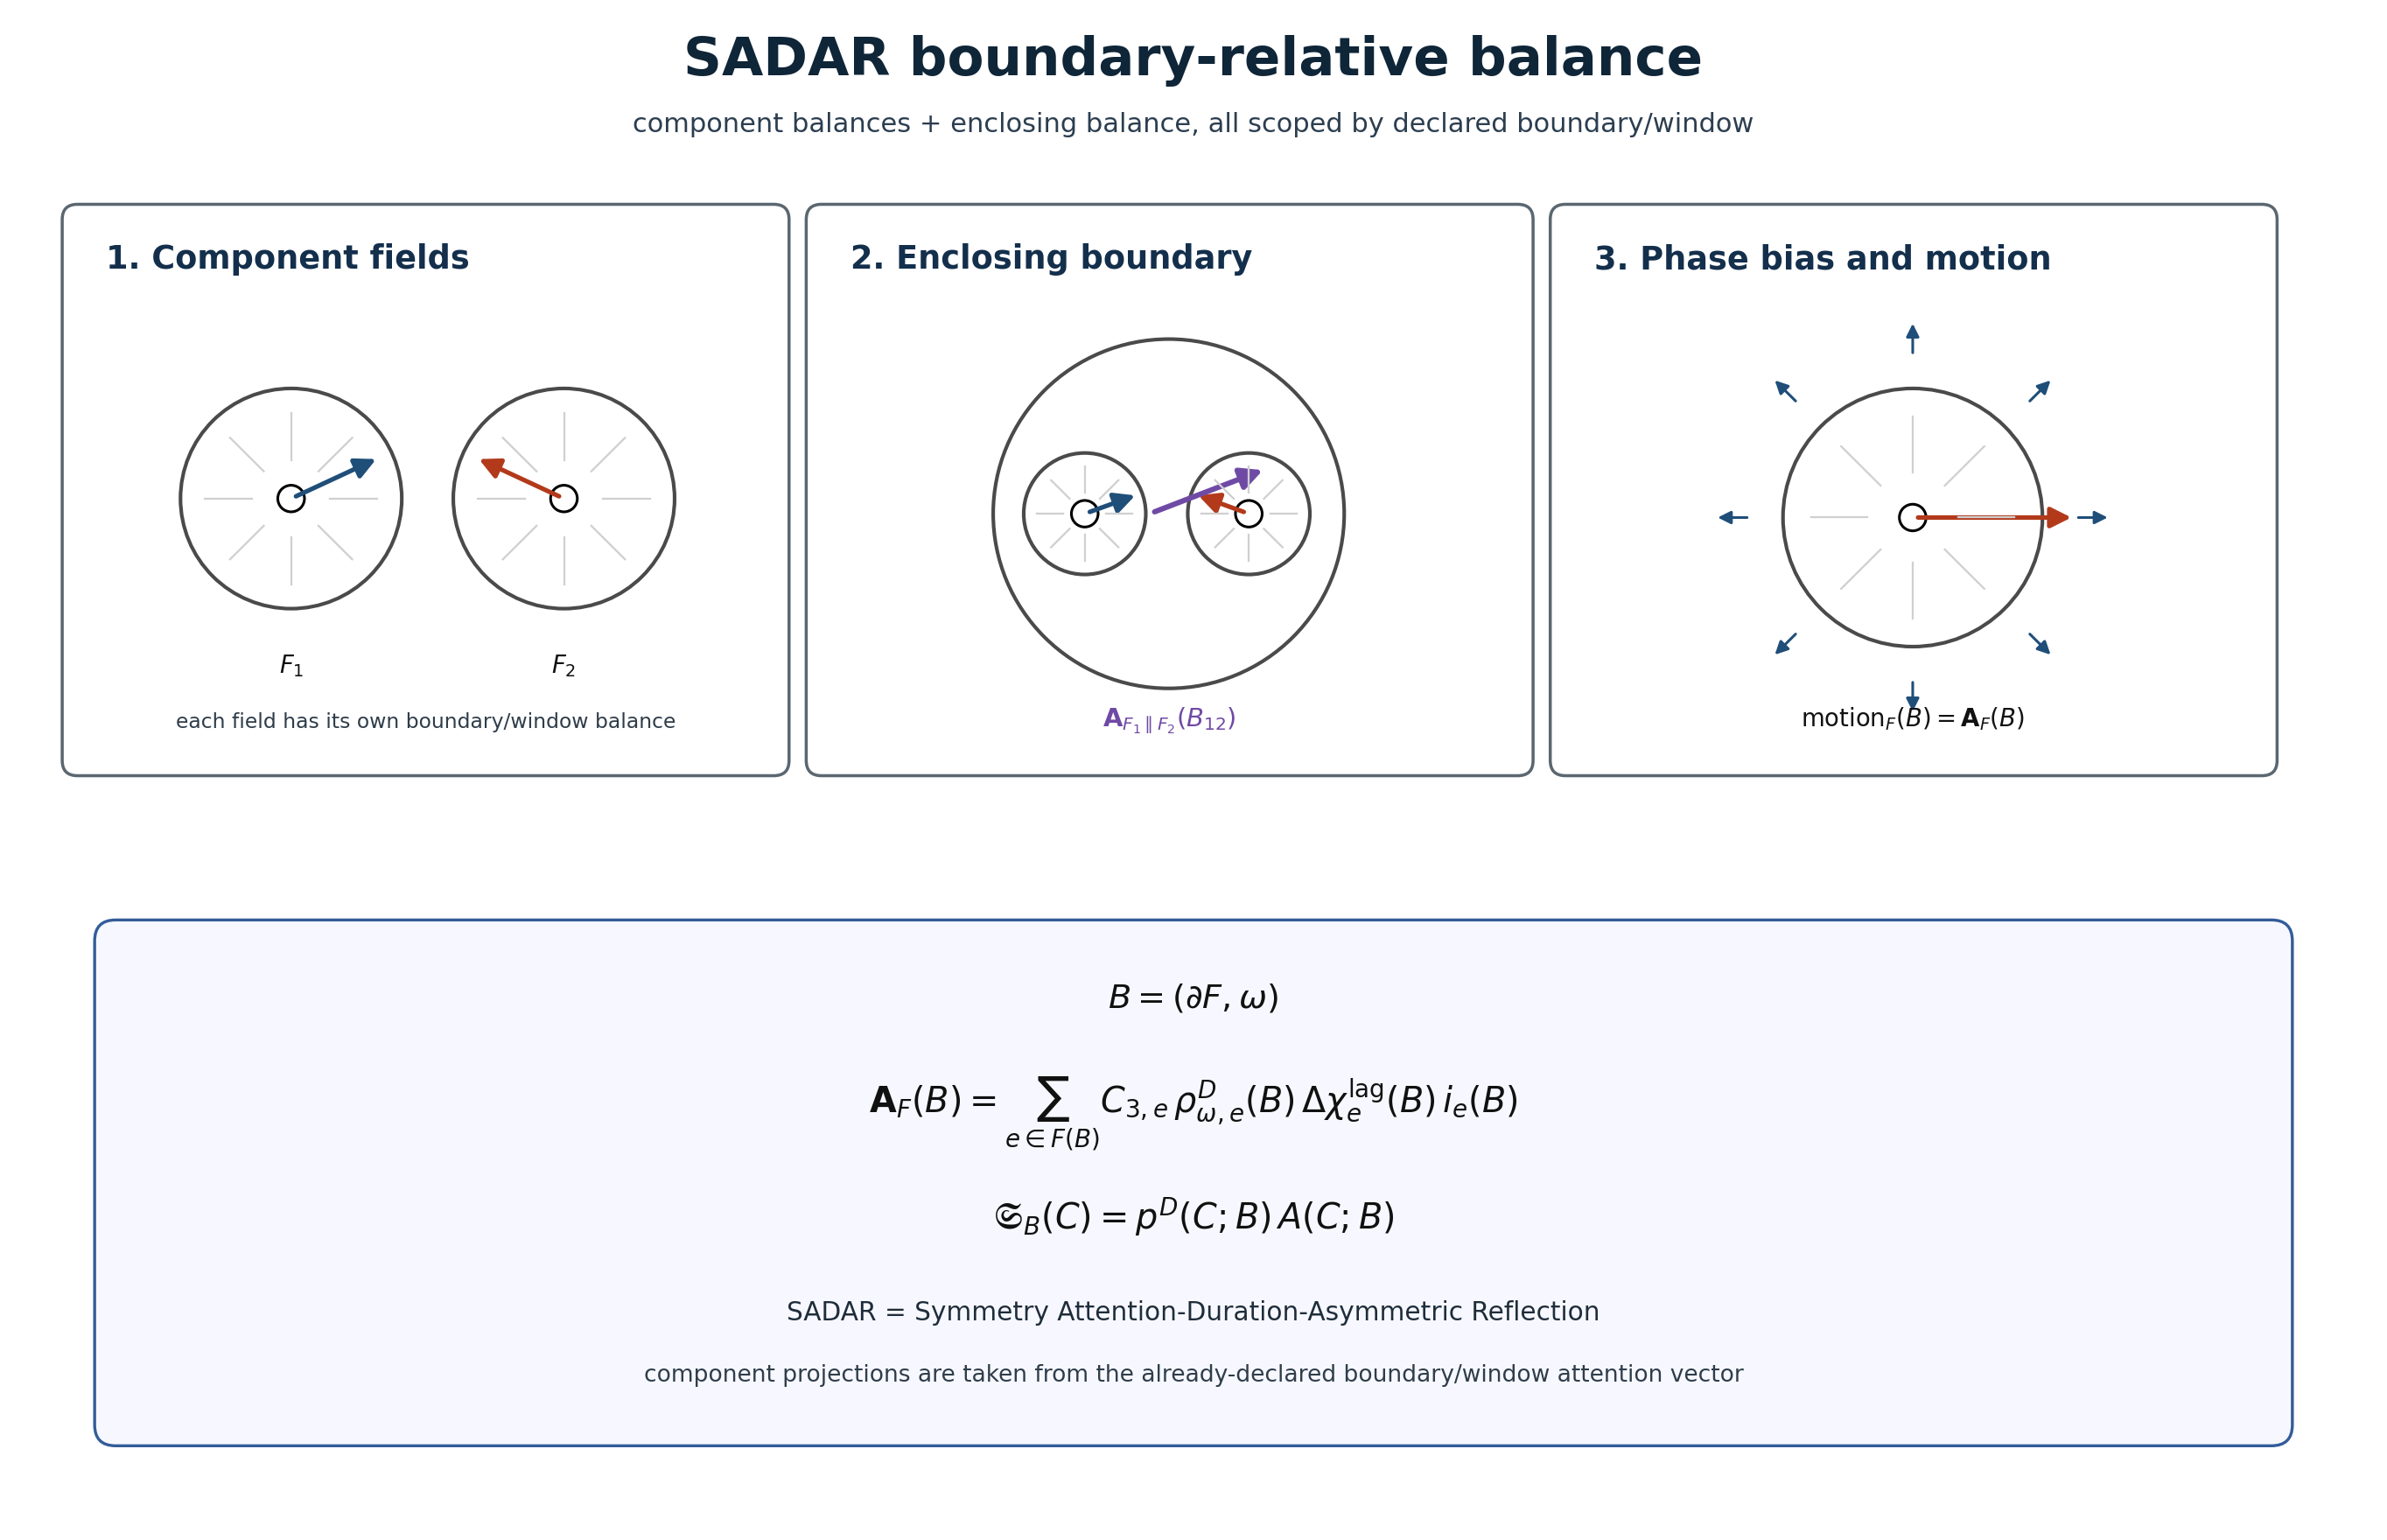
\includegraphics[width=0.94\linewidth]{figures_jpg/sadar_boundary_relative_balance.png}
\caption{SADAR boundary-relative balance. Component fields carry local SADAR attention vectors on their own declared boundaries. An enclosing boundary binds them as a super-field with its own SADAR attention vector. Phase bias shifts the boundary/window-specific SADAR balance; unresolved excess follows a sheddic path.}
\label{fig:sadar-boundary-relative-balance}
\end{figure}

\subsubsection{Sheddic route reference}\label{subsec:sadar-sheddic-route-reference}
Shedding is unresolved excess from the current SADAR balance. Unresolved excess follows a sheddic path. The sheddic excess is defined in \eqnref{eq:shedding-excess}, and the sheddic path route is fixed by \eqnref{eq:sheddic-path}.

\subsubsection{Component projection}\label{subsec:component-projection}
Component projections select declared components of the already-fixed SADAR attention vector.

\aodprovenance{\eqnref{eq:adar-channel},
\eqnref{eq:sadar-field},
\eqnref{eq:sadar-attention-vector},
\eqnref{eq:rcd-coupling},
\eqnref{eq:motion-sadar-attention},
\eqnref{eq:incident-return-shift},
\eqnref{eq:matched-return-cancellation},
\eqnref{eq:sheddic-path},
\appref{app:curling-curls}.}

\subsection{Cycle-shedding and temporal SADAR burden}\label{sec:cycle-shedding-temporal-sadar-burden}

\subsubsection{Temporal cycle group}\label{subsec:temporal-cycle-group}
\begin{definition}[Temporal cycle group]
A temporal cycle group is a carried segment of duon current participating in wave continuity. \appref{app:wave}.
\end{definition}

\subsubsection{Lead-lag burden}\label{subsec:lead-lag-burden}
\begin{definition}[Lead--lag disturbance span]
The lead--lag disturbance span is the carried asymmetric return extent of a temporal cycle group on the declared cut lineage.
\end{definition}

\subsubsection{Temporal SADAR burden}\label{subsec:temporal-sadar-burden}
For a temporal cycle group \(W\) on a declared boundary/window, its temporal SADAR burden is
\begin{equation}
P^{\SADARop}_{W}(\partial F,\omega)=
\sum_{e\in W}
C_{3,e}
\rho^D_{\omega,e}(\partial F,\omega)
\left|\Delta^{\chi\mathrm{lag}}_e\right|.
\label{eq:temporal-sadar-burden}
\end{equation}
This burden is taken up by SADAR balance in \secref{sec:field:sadar}.

\subsubsection{Shedding}\label{subsec:shedding}
\begin{definition}[Shedding]
Shed is the verb. Shedding is the direction-neutral noun for the parent surplus process. Sheddic is the adjective for path, route, value, and audit descriptors. Endoshedding and exoshedding carry directionality.

Shedding is the break of excess carried disturbance from local closure compatibility. If \(C^{\mathrm{close}}_W(\partial F,\omega)\) is local closure compatibility, then
\begin{equation}
\Delta_{\mathrm{close}}(\partial F,\omega)
=
P_W^{\SADARop}(\partial F,\omega)-C^{\mathrm{close}}_W(\partial F,\omega).
\label{eq:closure-residual}
\end{equation}
\begin{equation}
X_{\mathrm{shedding}}(\partial F,\omega)=
\max\!\left(0,
\Delta_{\mathrm{close}}(\partial F,\omega)
\right)
\label{eq:shedding-excess}
\end{equation}
records sheddic excess. A negative closure residual is a deficit/open check, not sheddic surplus.
\end{definition}

\subsubsection{Sheddic path}\label{subsec:sheddic-path}
Shedding is unresolved excess from local closure compatibility. Unresolved excess follows a sheddic path. The path may pass through \(E_2\), \(\mathsf C_6\), \(\mathsf C_8\), \(\mathsf C_{10}\), or a higher even enclosure form \(\mathsf C_{2n}\); seat-compatible retention determines which form is retained on the declared boundary/window:
\begin{equation}
\mathrm{SheddicPath}(X_{\mathrm{shedding}})
\in
\{E_2,\mathsf C_6,\mathsf C_8,\mathsf C_{10},\ldots,\mathsf C_{2n}\}.
\label{eq:sheddic-path}
\end{equation}
After a route partition is declared, the parent surplus may be placed as
\begin{equation}
X_{\mathrm{shedding}}
=
X_{\mathrm{endo}}+X_{\mathrm{exo}}+X_{\mathrm{redir}}+X_{\mathrm{open}}.
\label{eq:shedding-route-partition}
\end{equation}
Here \(X_{\mathrm{endo}}\) is endoshedding, \(X_{\mathrm{exo}}\) is exoshedding, \(X_{\mathrm{redir}}\) is redirected support routing, and \(X_{\mathrm{open}}\) is unretained open loss. Shedding is the parent surplus; endoshedding, exoshedding, redirected support routing, and open loss are route placements of \(X_{\mathrm{shedding}}\) after \(\operatorname{SheddicPath}\) is declared.
With reclosure fraction \(\lambda_{\mathrm{reclose}}\in[0,1]\), write
\[
X_W^{\mathrm{reclose}}=\lambda_{\mathrm{reclose}} X_{\mathrm{shedding}},
\qquad
X_W^{\mathrm{out}}=(1-\lambda_{\mathrm{reclose}})X_{\mathrm{shedding}}.
\]
Here \(X_W^{\mathrm{out}}\) is the non-reclosed outward remainder. After route placement,
\[
X_W^{\mathrm{out}}=X_{\mathrm{exo}}+X_{\mathrm{redir}}+X_{\mathrm{open}}.
\]
A sheddic path may reclose, continue outward, or carry decay status according to seat-compatible retention and support-enclosure compatibility.


\subsubsection{Yro odd-window route-status suffix}\label{subsec:yro-odd-window-route-status}
For an odd declared window length \(L=2k+1\), write
\[
\operatorname{Yro}_{L}(K;B).
\]
This is an odd-window unstable route-status suffix for a compact curling-curl specification \(K\) on the declared boundary/window \(B\). It records route status between adjacent even support enclosures \(\mathsf C_{2k}\) and \(\mathsf C_{2k+2}\). The support-enclosure ladder remains the even sequence
\[
\mathsf C_6,\ \mathsf C_8,\ \mathsf C_{10},\ldots,\mathsf C_{2n}.
\]
The yro status may be driven by surplus, deficit, pending overhang, hinge slide, seat-compatible retention cutoff, terminal split, or another declared route instability. The construction trace and sheddic-route audit fix which condition applies on the declared scope.

\paragraph{Naming audit.}
A yro suffix is audited as route status on a declared boundary/window and is recorded separately from support-enclosure names.

\subsubsection{Entropic duon current}\label{sec:entropic-duon-current}
\begin{definition}[Entropic duon current]
Entropic duon current is retained duon current carrying unresolved return burden. It carries retained ternary capacity through shell return, shedding, reclosure, and SADAR dynamics.
\end{definition}
For a declared field, boundary, and window, one local scalar form is
\begin{equation}
J^D_{\mathrm{ent}}(\partial F,\omega)=
\sum_{e\in F(\partial F,\omega)}
C_{3,e}
\rho^D_{\omega,e}(\partial F,\omega)
\left|\Delta^{\chi\mathrm{lag}}_e\right|.
\label{eq:entropic-duon-current}
\end{equation}
Entropic duon current carries unresolved temporal-cycle burden retained in duon current. Coherent wave continuity may accumulate lead--lag excess; retained excess contributes to entropic duon current.

\begin{figure}[H]
\centering
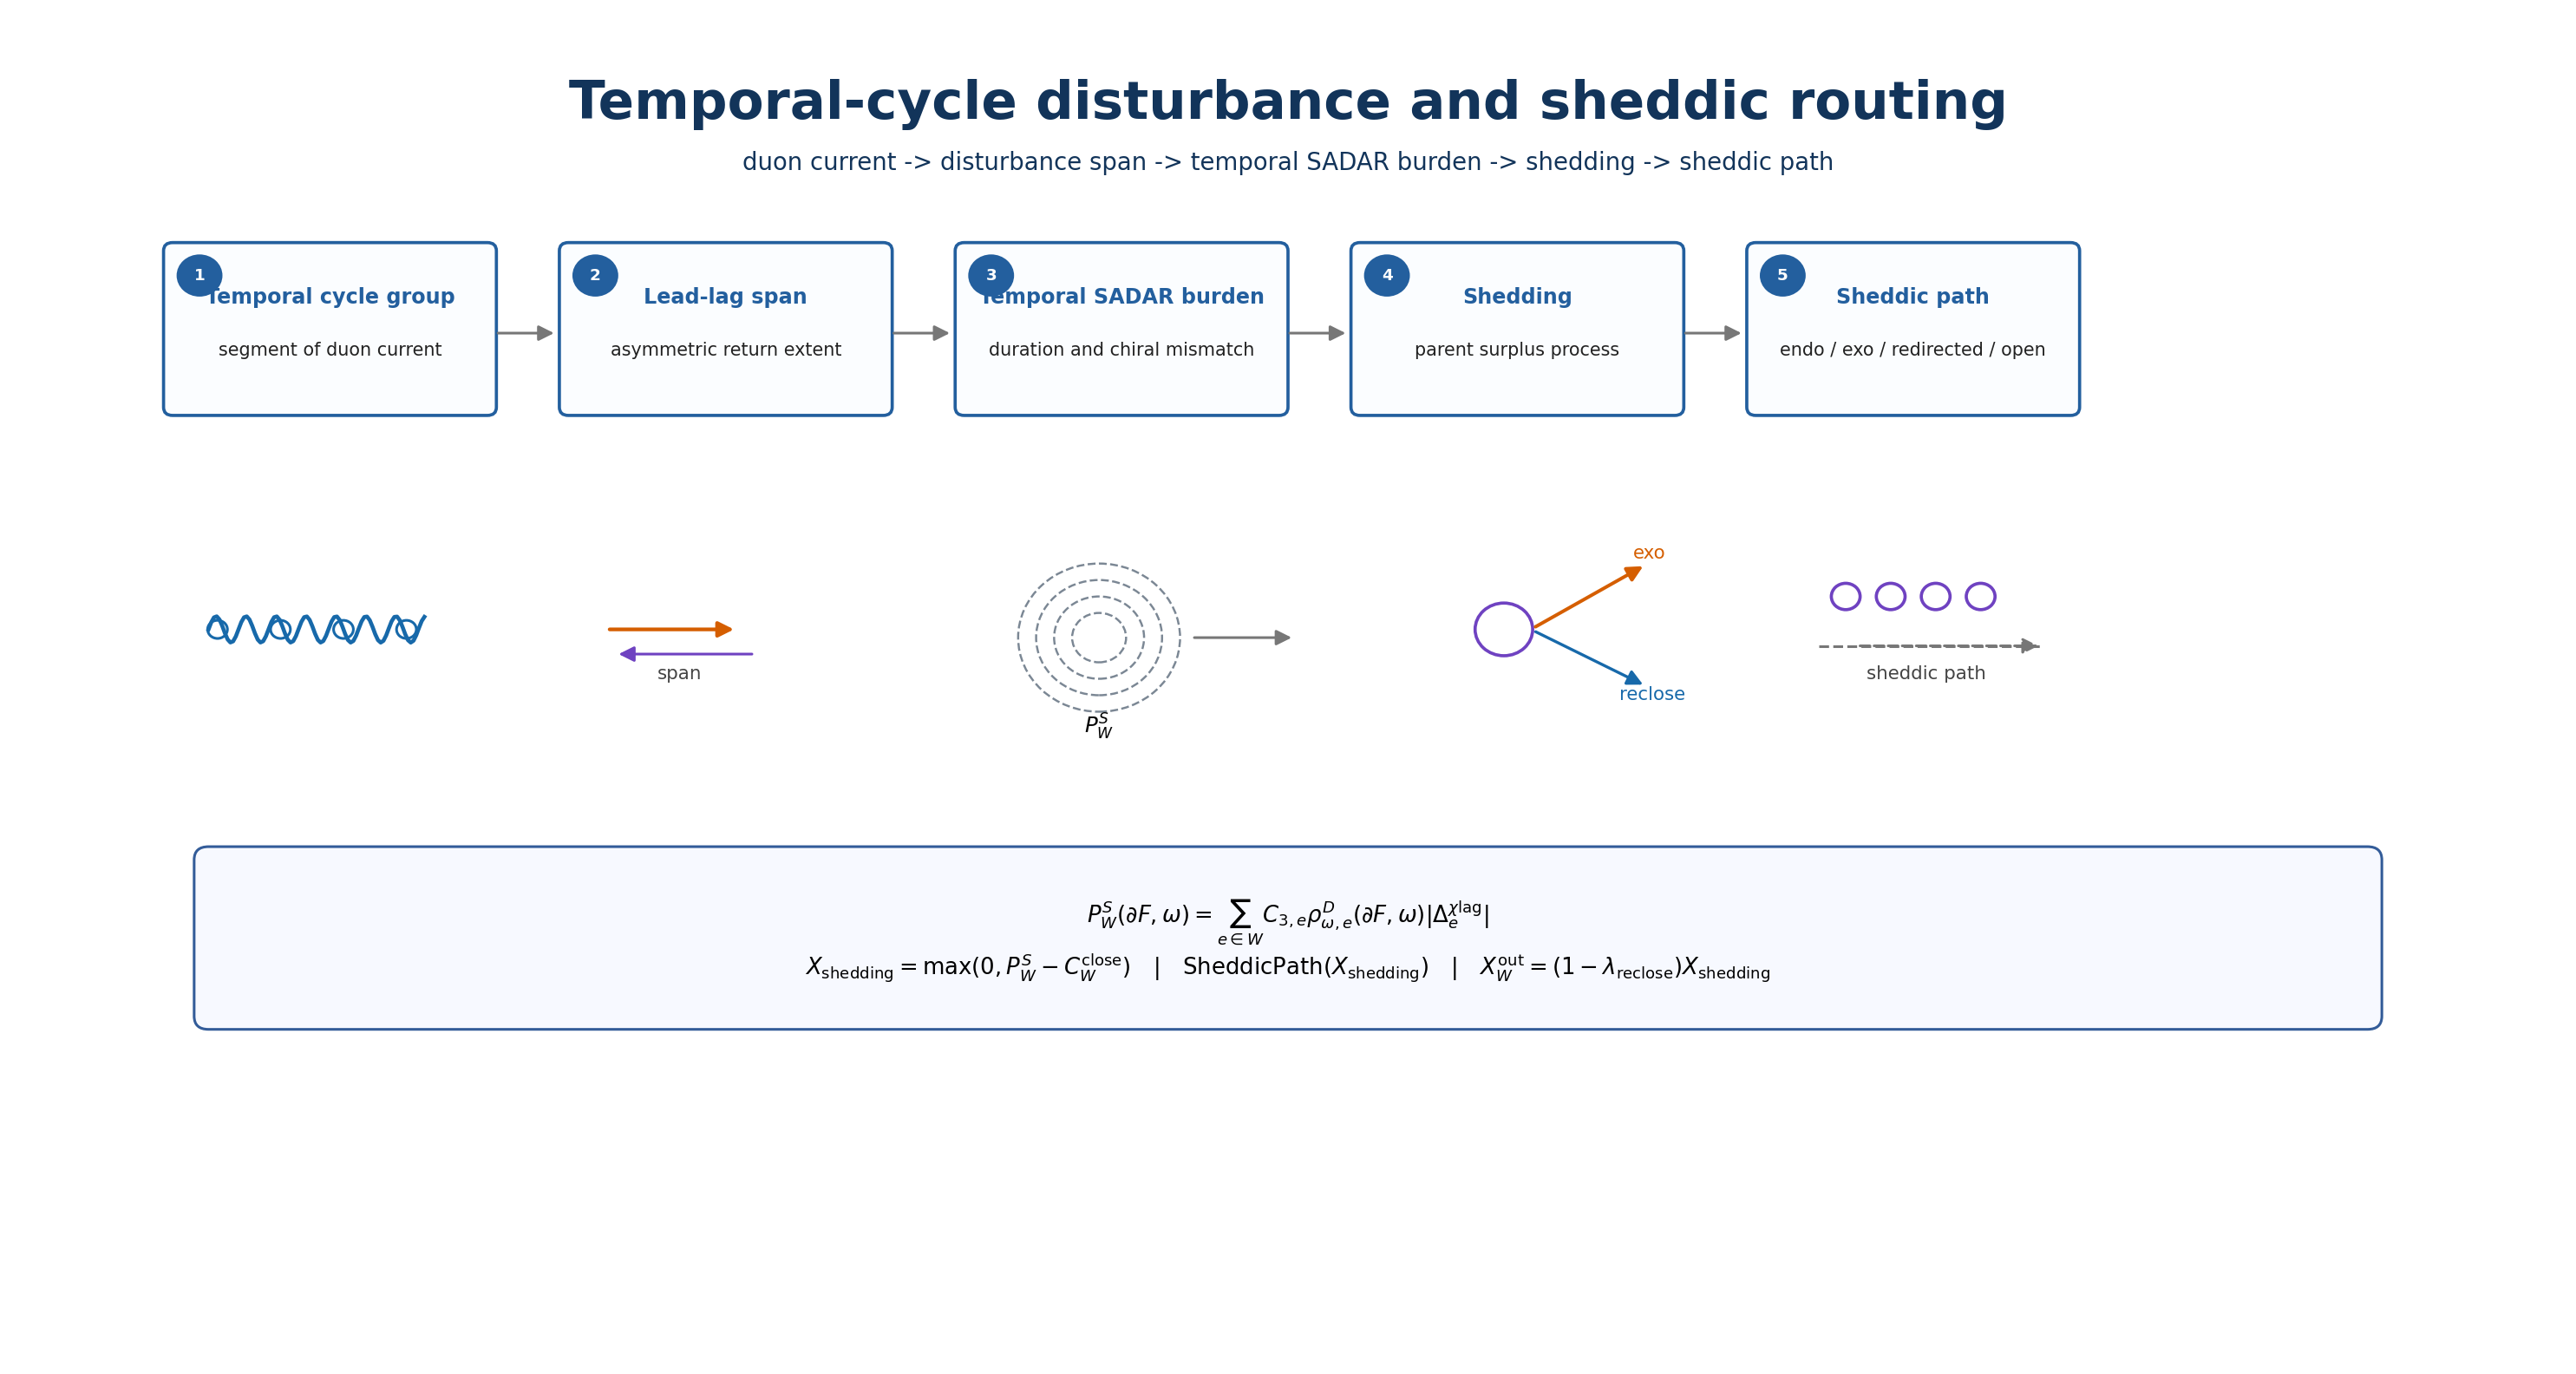
\includegraphics[width=0.96\linewidth]{figures_jpg/cycle_disturbance_shedding.png}
\caption{Temporal cycle lead--lag disturbance and shedding.}
\label{fig:v39-cycle-disturbance-shedding}
\end{figure}

\aodprovenance{\eqnref{eq:duon-current},
\eqnref{eq:returned-duration},
\eqnref{eq:temporal-sadar-burden},
\eqnref{eq:shedding-excess},
\eqnref{eq:sheddic-path},
\eqnref{eq:sadar-attention-vector},
\eqnref{eq:entropic-duon-current},
\eqnref{eq:sadar-field},
\eqnref{eq:support-enclosure-excess},
\appref{app:wave},
\appref{app:curling-curls}.}

\subsection{Seat compatibility and shell/enclosure routing}\label{sec:seat-shell-enclosure-routing}

\subsubsection{Even sequence}\label{subsec:support-enclosure-even-sequence}
The even sequence separates the current-side double form, the inner enclosure, and the outer enclosures.

\subsubsection{E2 duon}\label{subsec:e2-duon}
\[
E_2=\mathrm{duon},
\qquad
E_2^0=\text{open-seat duon}.
\]

\subsubsection{E2\texorpdfstring{\(^{\pm}\)}{±} duad}\label{subsec:e2-duad}
\[
E_2^{\pm}=\mathrm{duad}.
\]
Duad is the seated state of \(E_2\).

\subsubsection{E4 tetron}\label{subsec:e4-tetron}
\[
E_4=\mathrm{tetron}.
\]
Tetron is the default inner enclosure with four seats.

\subsubsection{Outer enclosures}\label{subsec:outer-enclosures}
A support enclosure is an outer even enclosure available to shell/enclosure routing:
\[
\mathsf C_{2m}=\text{support enclosure of order }2m,
\qquad m\ge3.
\]

\subsubsection{Hexon}\label{subsec:hexon}
\[
\mathsf C_6=\mathrm{hexon}.
\]
Hexon is the first outer enclosure because the hinge triad supplies left/right threefold closure: \(\mathsf H_3+\mathsf H_3=6\).

\subsubsection{Octon}\label{subsec:octon}
\[
\mathsf C_8=\mathrm{octon}.
\]

\subsubsection{Decon}\label{subsec:decon}
\[
\mathsf C_{10}=\mathrm{decon}.
\]

\subsubsection{Higher even enclosures}\label{subsec:higher-even-enclosures}
Higher even enclosures continue the outer sheddic path sequence:
\[
\mathsf C_{2n},
\qquad n>5.
\]
Outer enclosures are retained forms of sheddic paths. Hexon is the first outer enclosure; octon and decon are higher sheddic path forms; \(\mathsf C_{2n}\) records the higher even sequence.

\subsubsection{Filled shared enclosure}\label{subsec:filled-shared-enclosures}
A filled shared enclosure has
\[
m:m:0::2m,
\qquad m\ge3.
\]
Examples:
\[
3:3:0::6=\mathrm{Tritrio}^{3}::\mathrm{Tetratrio}^{3}::\mathrm{hexon},
\]
\[
4:4:0::8=\mathrm{Tritrio}^{4}::\mathrm{Tetratrio}^{4}::\mathrm{octon},
\]
\[
5:5:0::10=\mathrm{Tritrio}^{5}::\mathrm{Tetratrio}^{5}::\mathrm{decon}.
\]

\subsubsection{Closure excess}\label{subsec:support-enclosure-sadar-closure}
For a support-enclosure declaration \(\mathcal C=a:b:c::L\) on \(B=(\partial F,\omega)\), shell/enclosure routing carries the already-declared sheddic excess on the available route \(\mathcal C\). The routed closure excess is
\begin{equation}
X_{\mathcal C}(B)
=
\operatorname{route}_{\mathcal C}\!\left(X_{\mathrm{shedding}}(B)\right).
\label{eq:support-enclosure-excess}
\end{equation}
The value and placement of \(X_{\mathcal C}\) determine local rebalancing, exoshedding, endoshedding, or redirected support routing.

\subsubsection{Seat-compatible retention duration}\label{subsec:support-enclosure-retention-condition}
For a support-enclosure declaration \(\mathcal C=a:b:c::L\), write
\begin{equation}
\mathrm{TTL}_{\mathcal C}(\partial F,\omega)
=
\text{retained tick duration available for seat-compatible SADAR rebalancing}.
\label{eq:support-enclosure-retention}
\end{equation}
This is distinct from \(\rho^D_{\omega,ij}(B)\), the window-clipped duration participation clip for a channel.
Retention on the declared window is \(\mathrm{TTL}_{\mathcal C}(\partial F,\omega)\ge |\omega|\). If \(\mathrm{TTL}_{\mathcal C}(\partial F,\omega)<|\omega|\), the sheddic path continues through re-entry, reclosure, or decay status before the window closes.

\begin{figure}[H]
\centering
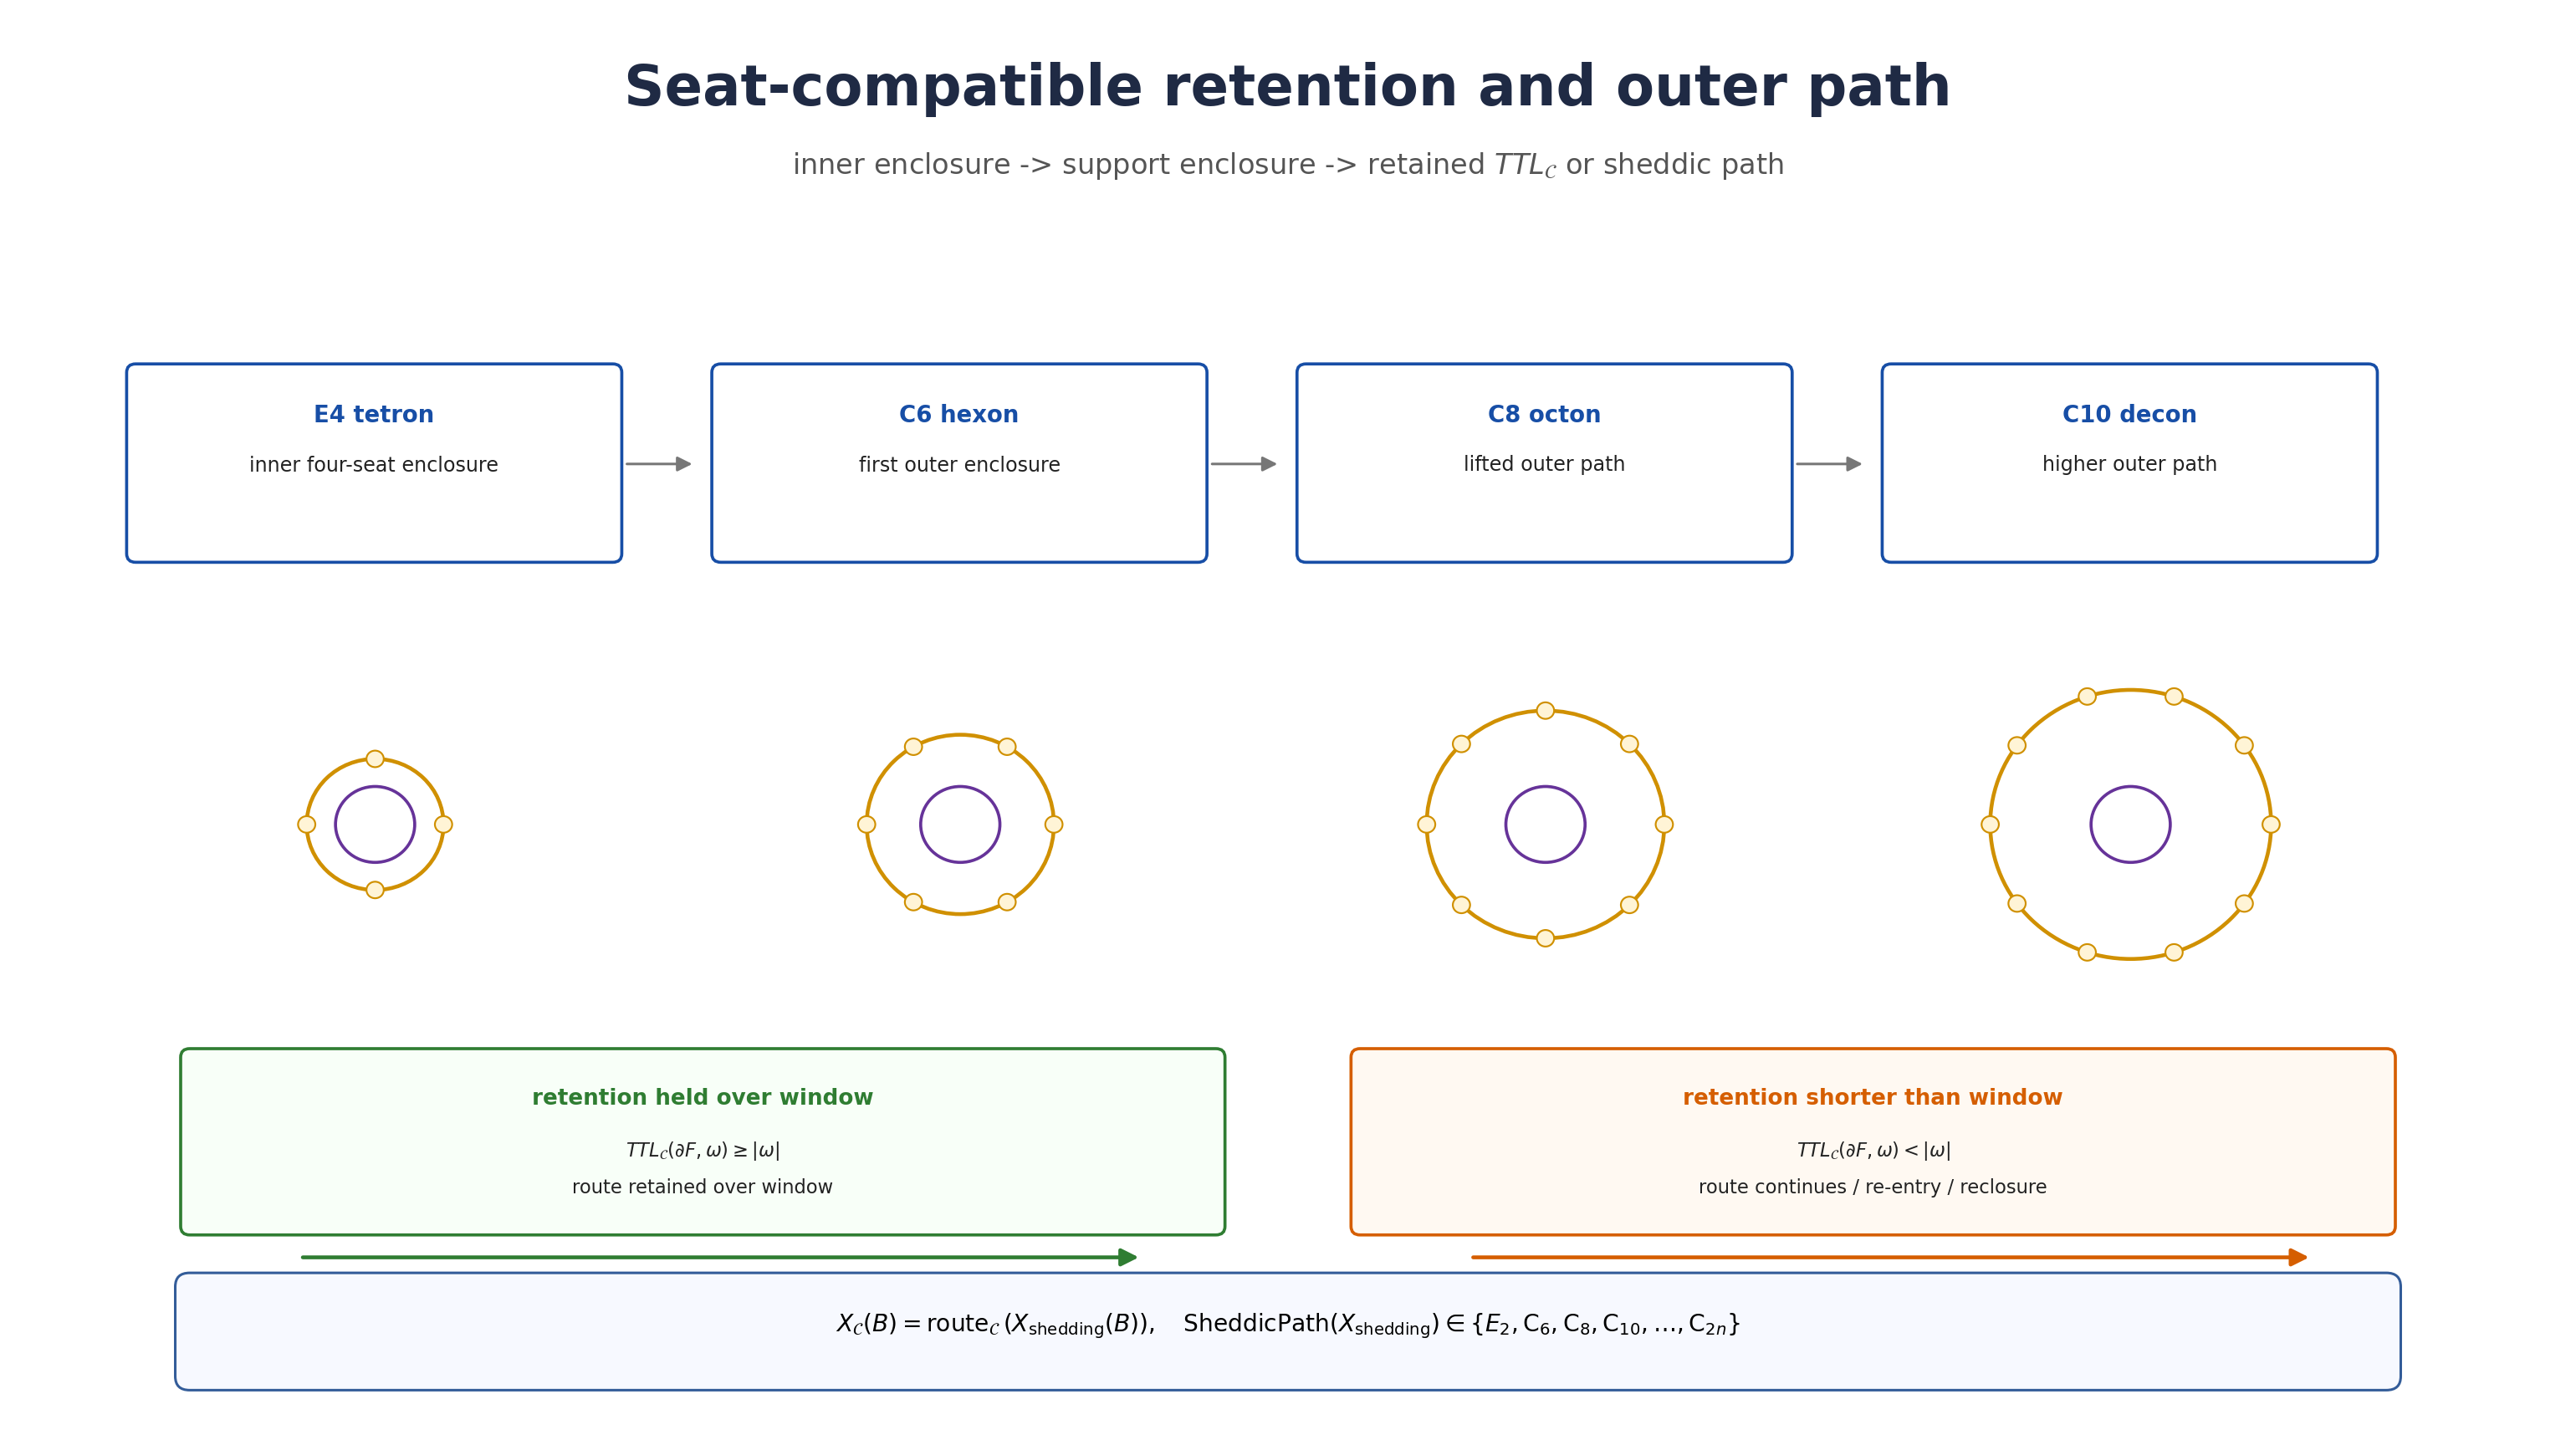
\includegraphics[width=0.96\linewidth]{figures_jpg/support_enclosure_retention.png}
\caption{Seat compatibility and support-retention duration for sheddic paths.}
\label{fig:support-enclosure-retention}
\end{figure}

\subsubsection{Coord-0 grouping}\label{subsec:coord-zero-support-enclosure-grouping}
At coordinate \(0\), write coord-0 shell-stack declarations as
\[
0\mid-::Z:A:0:L\langle a:b:c::L\rangle.
\]
For filled support-enclosure grouping,
\[
0\mid-::Z:A:0:2m\langle m:m:0::2m\rangle.
\]
Define the cumulative group boundary
\[
\Gamma_m=\sum_{k=3}^{m}2k=m(m+1)-6,
\qquad
\Gamma_2=0.
\]
Then \(\Gamma_{m-1}<Z\le \Gamma_m\) selects the coord-0 support-enclosure group.

\aodprovenance{\eqnref{eq:sadar-field},
\eqnref{eq:support-enclosure-excess},
\eqnref{eq:support-enclosure-retention},
\appref{app:curling-curls}.}


\subsection{Shell paths}\label{sec:shell-paths}

\subsubsection{Shared shell-path declaration}\label{subsec:shared-shell-path-declaration}
The shared shell-path declaration may be written
\[
0\mid-::Z:A:0:6\langle 1:1:0::6\rangle.
\]
Named:
\[
0\mid-::Z:A:0:\mathrm{hexon}\langle \mathrm{Tritrio}::\mathrm{Tetratrio}::\mathrm{hexon}\rangle.
\]
For the filled hexon field, write
\[
0\mid-::Z:A:0:6\langle 3:3:0::6\rangle.
\]
Named:
\[
0\mid-::Z:A:0:\mathrm{hexon}\langle \mathrm{Tritrio}^{3}::\mathrm{Tetratrio}^{3}::\mathrm{hexon}\rangle.
\]

\subsubsection{Nested shell-stack pattern}\label{subsec:nested-shell-stack-pattern}
The same curling-curl pattern iterates upward through shared enclosures and filled enclosures:
\[
\mathrm{Tritrio}^{3}::\mathrm{Tetratrio}^{3}::\mathrm{hexon}
\to
\mathrm{Tritrio}^{4}::\mathrm{Tetratrio}^{4}::\mathrm{octon}
\to
\mathrm{Tritrio}^{5}::\mathrm{Tetratrio}^{5}::\mathrm{decon}.
\]

\subsubsection{Shell-path closure references}\label{subsec:shell-path-closure-references}
Shell-path closure fixtures are recorded in \appref{app:combinatorics-rd-tests} and \appref{app:path-complexity-quarantine}. The core pressure calculation remains
\[
p^D_{ij}(B)=C_{3,ij}\rho^D_{\omega,ij}(B),
\qquad
\phi_{ij}(B)=p^D_{ij}(B)A_{ij}(B).
\]


\subsection{Fusion closure and chain reclosure}\label{sec:fusion-closure-chain-reclosure}

\subsubsection{Fusion closure}\label{subsec:fusion-closure}
Fusion is branch/hinge/branch closure of admitted curling-curl support forms. For admitted forms \(F\) and \(G\), define
\begin{equation}
\operatorname{Fuse}_{B}(F,G)
:=
\operatorname{Close}_{B}
\left(
\widehat F\;\mu\;\widehat G
\right),
\label{eq:fusion-closure}
\end{equation}
where \(\widehat F=\operatorname{Compress}(F)\) and \(\widehat G=\operatorname{Compress}(G)\). Closed forms fuse; exposed fragments do not.

The branch/hinge/branch fusion duration is
\begin{equation}
RD_{\mathrm{fuse}}(F,G;B)
=
\Pi^-_{\widehat F}(B)+H_{\mu,\widehat F,\widehat G}(B)+\Pi^+_{\widehat G}(B).
\label{eq:fusion-branch-hinge-duration}
\end{equation}

For a closure rung,
\begin{equation}
F_{n+1}
=
\operatorname{Close}_{B_{n+1}}
\left(
\widehat F_n\;\mu\;\widehat G_n
\right).
\label{eq:fusion-ladder-rung}
\end{equation}
The rung residual is
\begin{equation}
S_{n+1}=P^D_{n+1}-C_{\mathrm{close},n+1}.
\label{eq:fusion-rung-residual}
\end{equation}
If \(S_{n+1}>0\), the rung is surplus-producing; if \(S_{n+1}=0\), it is neutral retained; if \(S_{n+1}<0\), it is deficit/open. The sheddic surplus is
\begin{equation}
X_{\mathrm{shedding},n+1}=\max(0,S_{n+1}).
\label{eq:fusion-rung-shedding-surplus}
\end{equation}

\subsubsection{Exoshedding lift}\label{subsec:exoshedding-lift}
Exoshedding routes surplus support outside the current closure. At scope \(B_r\), nonzero \(X_{\mathrm{exo},r}\) supplies proposed lifted support
\begin{equation}
K^{r+1}_{\mathrm{prop}}
=
\operatorname{Lift}_{B_r\to B_{r+1}}
\left(X_{\mathrm{exo},r}\right).
\label{eq:exoshedding-lift}
\end{equation}
The construction trace admits it by
\begin{equation}
K^{r+1}_{\mathrm{prop}}
\xrightarrow{\,HT(K;B_{r+1})\,}
K^{r+1}_{\mathrm{adm}}(B_{r+1}).
\label{eq:lifted-support-admission}
\end{equation}
Higher-scope fusion closes the admitted lifted support:
\begin{equation}
F_{r+1}
=
\operatorname{Close}_{B_{r+1}}
\left(
\widehat F_r\;\mu\;K^{r+1}_{\mathrm{adm}}(B_{r+1})
\right).
\label{eq:higher-scope-fusion}
\end{equation}
Thus exoshedding supplies lifted support; fusion closes it.

\subsubsection{Link-closure ladder}\label{subsec:link-closure-ladder}
Chain reclosure is iterated higher-scope fusion over admitted supports routed by exoshedding. A local adjacent link closure is
\begin{equation}
L_{i,i+1}
=
\operatorname{Close}_{B_{i,i+1}}
\left(
\widehat F_i\;\mu\;\widehat F_{i+1}
\right).
\label{eq:link-closure-ladder}
\end{equation}
Its residual is
\begin{equation}
\Delta_{\mathrm{link}}=P^D_{\mathrm{link}}-C_{\mathrm{close,link}},
\qquad
X_{\mathrm{shedding},\mathrm{link}}=\max(0,\Delta_{\mathrm{link}}).
\label{eq:link-closure-residual}
\end{equation}

\aodprovenance{\secref{subsec:curling-curl-support-forms}, \secref{subsec:sheddic-path}, \eqnref{eq:branch-hinge-rd}.}


\subsection{Fractal Field Ring Gate}\label{subsec:fractal-field-ring-gate}
\aodnoteblock{Scope}{A fractal field ring gate is a declared recurrence motif on \(B=(\partial_TF,\omega)\).}

Declare
\begin{equation}
\mathfrak a\subset \mathcal A^{\mathrm{ret}}_8,
\qquad
B=(\partial_TF,\omega).
\label{eq:frg-scope}
\end{equation}
The AF recurrence is typed here: the distinctions are declared in \eqnref{eq:frg-distinctions}; the relations are declared in \eqnref{eq:frg-ring-adjacency}--\eqnref{eq:frg-return-relation}; the retained relation family is the FRG; \(\SADARop_B\) forms the A\(\Omega\) value.

\subsubsection{Distinctions}\label{subsec:frg-distinctions}
Declare
\begin{equation}
D_{\mathrm{FRG}}
=
(\mathfrak a,\ B,\ R_{\mathrm{ring}},\partial_T R_{\mathrm{ring}},V_N,I,G,K_{\mathrm{bin}},\kappa).
\label{eq:frg-distinctions}
\end{equation}
with
\[
V_N=\{0,1,\ldots,N-1\},
\qquad
R_{\mathrm{ring}}\subset F,
\]
\[
\partial_T R_{\mathrm{ring}}
=
\text{the tesseract-admissible boundary induced on }R_{\mathrm{ring}},
\]
\[
I\subseteq V_N,
\qquad
G=\{g_i:i\in I\},
\qquad
g_i\in\partial_T R_{\mathrm{ring}},
\]
\[
k\in K_{\mathrm{bin}},
\qquad
\kappa:K_{\mathrm{bin}}\to\mathbb Q,
\qquad
\kappa_k:=\kappa(k).
\]

\subsubsection{Relations}\label{subsec:frg-relations}
The ring adjacency relation is
\begin{equation}
E_N=
\{(i,i+1\bmod N),(i,i-1\bmod N):i\in V_N\}.
\label{eq:frg-ring-adjacency}
\end{equation}
The returned-current relation is
\begin{equation}
E_{\mathrm{return}}\subseteq I\times I.
\label{eq:frg-return-relation}
\end{equation}
For adjacent-only fixtures,
\begin{equation}
(i,j)\in E_{\mathrm{return}}
\Rightarrow
(i,j)\in E_N.
\label{eq:frg-adjacent-only-condition}
\end{equation}
Gate-to-bin and cross-return path relations are written directly as
\[
\gamma:g_i\leadsto k,
\qquad
\gamma:g_i\leftrightarrow g_j\leadsto k.
\]
The retained path-cycle carried by \(\gamma\) is \(C_\gamma\).

\subsubsection{Gate contribution}\label{subsec:frg-gate-contribution}
For a declared gate \(g_i\), define the bin contribution
\begin{equation}
S_k^{(i)}
=
\sum_{t\in\omega}
\sum_{\gamma:g_i\leadsto k}
\kappa_k\,
\SADARop_{B|t}(C_\gamma).
\tag{RG1}\label{eq:frg-gate-contribution}
\end{equation}

\subsubsection{Independent gate-sum value}\label{subsec:frg-independent-gate-sum}
The independent gate-sum value is
\begin{equation}
T_k^0=\sum_{i\in I}S_k^{(i)}.
\tag{RG2}\label{eq:frg-independent-gate-sum}
\end{equation}
For two gates,
\begin{equation}
T_k^0=S_k^{(a)}+S_k^{(b)}.
\tag{RG3}\label{eq:frg-independent-two-gate}
\end{equation}

\subsubsection{Cross-return contribution}\label{subsec:frg-cross-return-contribution}
For a returned-current pair \((i,j)\in E_{\mathrm{return}}\), define
\begin{equation}
C_{ij,k}^{\times}(B)
=
\sum_{t\in\omega}
\sum_{\gamma:g_i\leftrightarrow g_j\leadsto k}
\kappa_k\,
\SADARop_{B|t}(C_\gamma).
\tag{RG4}\label{eq:frg-cross-return-contribution}
\end{equation}
The two-gate specialization is
\begin{equation}
C_{ab,k}^{\times}(B)
=
\sum_{t\in\omega}
\sum_{\gamma:g_a\leftrightarrow g_b\leadsto k}
\kappa_k\,
\SADARop_{B|t}(C_\gamma).
\tag{RG5}\label{eq:frg-cross-return-two-gate}
\end{equation}

\subsubsection{Recurrent ring value}\label{subsec:frg-recurrent-ring-value}
The recurrent ring value is
\begin{equation}
T_k^\times
=
T_k^0+
\sum_{(i,j)\in E_{\mathrm{return}}}
C_{ij,k}^{\times}(B).
\tag{RG6}\label{eq:frg-recurrent-ring-value}
\end{equation}
For two gates,
\begin{equation}
T_k^\times=T_k^0+C_{ab,k}^{\times}(B).
\tag{RG7}\label{eq:frg-recurrent-two-gate}
\end{equation}

\subsubsection{Field-ring identity}\label{subsec:frg-identity}
The field-ring identity is
\begin{equation}
T_k^\times-T_k^0
=
\sum_{(i,j)\in E_{\mathrm{return}}}
C_{ij,k}^{\times}(B).
\tag{RG8}\label{eq:frg-identity}
\end{equation}
For two gates,
\begin{equation}
T_k^\times-T_k^0=C_{ab,k}^{\times}(B).
\tag{RG9}\label{eq:frg-identity-two-gate}
\end{equation}

\subsubsection{Exact-fixture corollary}\label{subsec:frg-delta-three-corollary}
If an exact fixture declares
\[
T_k^\times,O_k\in\mathbb Z,
\]
then record the exact ternary signed residual
\begin{equation}
\Delta_k^{\mathbb Z}=T_k^\times-O_k,
\qquad
s_k^{(3)}=\operatorname{sgn}(\Delta_k^{\mathbb Z})\in\{-1,0,+1\},
\qquad
m_k=|\Delta_k^{\mathbb Z}|\in\mathbb Z_{\ge0}.
\label{eq:frg-delta-three-components}
\end{equation}
Thus
\begin{equation}
\Delta_k^{\mathbb Z}=s_k^{(3)}m_k.
\label{eq:frg-delta-three-signed-product}
\end{equation}
The compact residual package is
\begin{equation}
\delta_{3,k}(T^\times,O)=(s_k^{(3)},m_k),
\qquad
\delta_3(T^\times,O)
=
\left(\delta_{3,k}(T^\times,O)\right)_{k\in K_{\mathrm{bin}}}.
\tag{RG10}\label{eq:frg-delta-three}
\end{equation}
Normalized decimal summaries belong to declared value maps or external comparison entries.

\subsubsection{FRG value package}\label{subsec:frg-value-package}
The compact FRG value package is
\begin{equation}
\mathcal V_{\mathrm{FRG}}
=
(\mathfrak a,\ B,\ R_{\mathrm{ring}},\partial_T R_{\mathrm{ring}},
V_N,E_N,I,G,K_{\mathrm{bin}},\kappa,E_{\mathrm{return}},\lambda_{\mathcal Y}).
\tag{RG11}\label{eq:frg-value-package}
\end{equation}
The declared value map is
\begin{equation}
\lambda_{\mathcal Y}:
(T_k^\times)_{k\in K_{\mathrm{bin}}}
\mapsto
\mathcal Y.
\tag{RG12}\label{eq:frg-value-map}
\end{equation}

\aodremark{FRG supplies gated recurrent cross-return; fusion closes admitted support.}

\subsection{Field dynamics}\label{sec:field-dynamics}

\subsubsection{Field-fluid regime}\label{subsec:field-fluid-regime}
Field dynamics is the A\(\Omega\)D calculation of retained field, current-cycle, background-continuation, and shell-support participants on declared \(B=(\partial_TF,\omega)\). A field-fluid regime is the local declaration in which those participants couple through finite SADAR capacity. For a moving or nested cell boundary, write
\[
B_c|t=(\partial_T R_c(t),\omega_c|t).
\]
The retained cycle family is
\[
\mathcal C_c(t)
=
\mathcal C_{\mathrm{field},c}
\cup
\mathcal C_{\mathrm{current},c}
\cup
\mathcal C_{\mathrm{bg},c}
\cup
\mathcal C_{\mathrm{shell},c}.
\]
Here
\[
C_J=\text{retained current-cycle participant},
\qquad
J^D=\text{accumulated current value}.
\]

\subsubsection{Cycle-beat resolution gate}\label{subsec:cycle-beat-resolution-gate}
Let
\[
\mathcal C_{a,r,\Sigma}
=
\operatorname{cycle}\langle a,r\rangle(\Sigma_{\mathrm{support}}),
\]
where \(\Sigma_{\mathrm{support}}\) is the declared support-expression family. The beat count is
\[
N_{\mathrm{beat}}(a,r,\Sigma;B)
=
\left|\operatorname{Sec}^{(r)}_{T,\mathrm{ret}}(a;B)\right|
\left|\Sigma_{\mathrm{support}}\right|.
\]
The monitored reflection-duration accessor is selected by the declared rule
\[
RD_{\mathrm{mon}}(a,r,\Sigma;B)
=
\max_{C_u\in\mathcal C_{a,r,\Sigma}}
RD_{\AO}(C_u;B).
\]
Resolution is chosen by a declared coarseness order \(\preceq_{\mathrm{coarse}}\). Tie-breakers are declared before application. The selected \(q\) is the coarsest admissible resolution under \(\preceq_{\mathrm{coarse}}\) after declared tie-breakers. No measured residual or score enters this gate.

\subsubsection{Medium declaration and field count}\label{subsec:medium-declaration-field-count}
Declare integer or rational constants before application. The raw maximum supported field count is
\[
N^{\max,0}_{F,c}
=
\min\left(
N_{\mathrm{candidate},c},
N_{\mathrm{beat},c},
\left\lfloor\frac{\mathcal K^{\mathrm{raw}}_c}{\bar k_F}\right\rfloor,
\left\lfloor\frac{|\omega_c|}{\bar\rho^D_F}\right\rfloor
\right).
\]
The retained field family is then declared as
\[
F_{B_c}=\{F_1,\ldots,F_{n_F(c)}\},
\qquad
n_F(c)\le N^{\max,0}_{F,c}.
\]
A gas/fluid classifier is a declaration on \(B_c\), not an external material label. Chiral flip, background-continuation jitter, slosh, semi-coupling, and lead-lag are boundary-current features of the declared regime.


\aodremark{A field-fluid regime may distinguish locally seated, unresolved-jitter, pending, and sheddic chiral events by declared boundary status. Application fixtures evaluate these distinctions as manual entries.}

\subsubsection{Nested boundary and inter-layer SADAR coupling}\label{subsec:interlayer-sadar-coupling}
For nested boundaries
\[
R_0\subset R_1\subset\cdots\subset R_m,
\qquad
B_\ell=(\partial_T R_\ell,\omega_\ell),
\]
the inter-layer coupling value is
\[
G^{\mathfrak S}_{\ell\to m}(B)
=
\sum_{(u,v)\in E^{\mathfrak S}_{\ell,m}(B)}
\SADARop_B(C_u,C_v).
\]
Range-prioritized coupling orders admissible \(E^{\mathfrak S}_{\ell,m}(B)\) by the declared boundary range before summation. When a magnitude is needed, use the declared magnitude functional
\[
J^{D,\mathrm{try}}_{r,c}
=
\sum_{(u,v)\in E_r(B_c)}
\left\|\SADARop_{B_c}(C_u,C_v)\right\|_{\mathrm{decl}}.
\]

\subsubsection{Capacity residual and exoshedding lift}\label{subsec:capacity-residual-exoshedding-lift}
The capacity residual and closure residual are
\[
\Delta^{\mathrm{cap}}_\ell=P^D_\ell-C^{\mathrm{cap}}_\ell,
\qquad
\Delta_{\mathrm{close},\ell}=P^D_\ell-C_{\mathrm{close},\ell}.
\]
The sheddic surplus is
\[
X_{\mathrm{shedding},\ell}=\max(0,\Delta_{\mathrm{close},\ell}),
\]
with declared route partition
\[
X_{\mathrm{shedding},\ell}=X_{\mathrm{endo},\ell}+X_{\mathrm{exo},\ell}+X_{\mathrm{redir},\ell}+X_{\mathrm{open},\ell}.
\]
Exoshedding supplies lifted support:
\[
X_{\mathrm{exo},\ell}>0
\Rightarrow
K_{\mathrm{prop}}^{\ell+1}
=
\operatorname{Lift}_{B_\ell\to B_{\ell+1}}
\left(X_{\mathrm{exo},\ell}\right).
\]
The lifted key is admitted by trace,
\[
K_{\mathrm{prop}}^{\ell+1}
\xrightarrow{HT(K;B_{\ell+1})}
K_{\mathrm{adm}}^{\ell+1}(B_{\ell+1}),
\]
and higher-scope fusion is
\[
F_{\ell+1}
=
\operatorname{Close}_{B_{\ell+1}}
\left(
\widehat F_\ell
\mu
K_{\mathrm{adm}}^{\ell+1}(B_{\ell+1})
\right).
\]

\subsubsection{FRG-mediated cross-return in nested boundaries}\label{subsec:frg-nested-boundary}
When a nested boundary is ring-gated, declare
\[
D_{\mathrm{FRG},\ell}
=
(B_\ell,V_{N_\ell},I_\ell,G_\ell,K_{\mathrm{bin},\ell},\kappa_\ell,E_{\mathrm{return},\ell}).
\]
The cross-return contribution is
\[
C_{ij,k}^{\times}(B_\ell)
=
\sum_{t\in\omega_\ell}
\sum_{\gamma:g_i\leftrightarrow g_j\leadsto k}
\kappa_k
\SADARop_{B_\ell|t}(C_\gamma),
\]
and the recurrent value is
\[
T_{\ell,k}^{\times}
=
T_{\ell,k}^{0}
+
\sum_{(i,j)\in E_{\mathrm{return},\ell}}
C_{ij,k}^{\times}(B_\ell).
\]
FRG supplies gated recurrent cross-return. Fusion closes admitted support. Exoshedding lifts surplus to a higher declared boundary. Chain reclosure is iterated higher-scope fusion, sometimes FRG-mediated.

\begin{figure}[H]
\centering
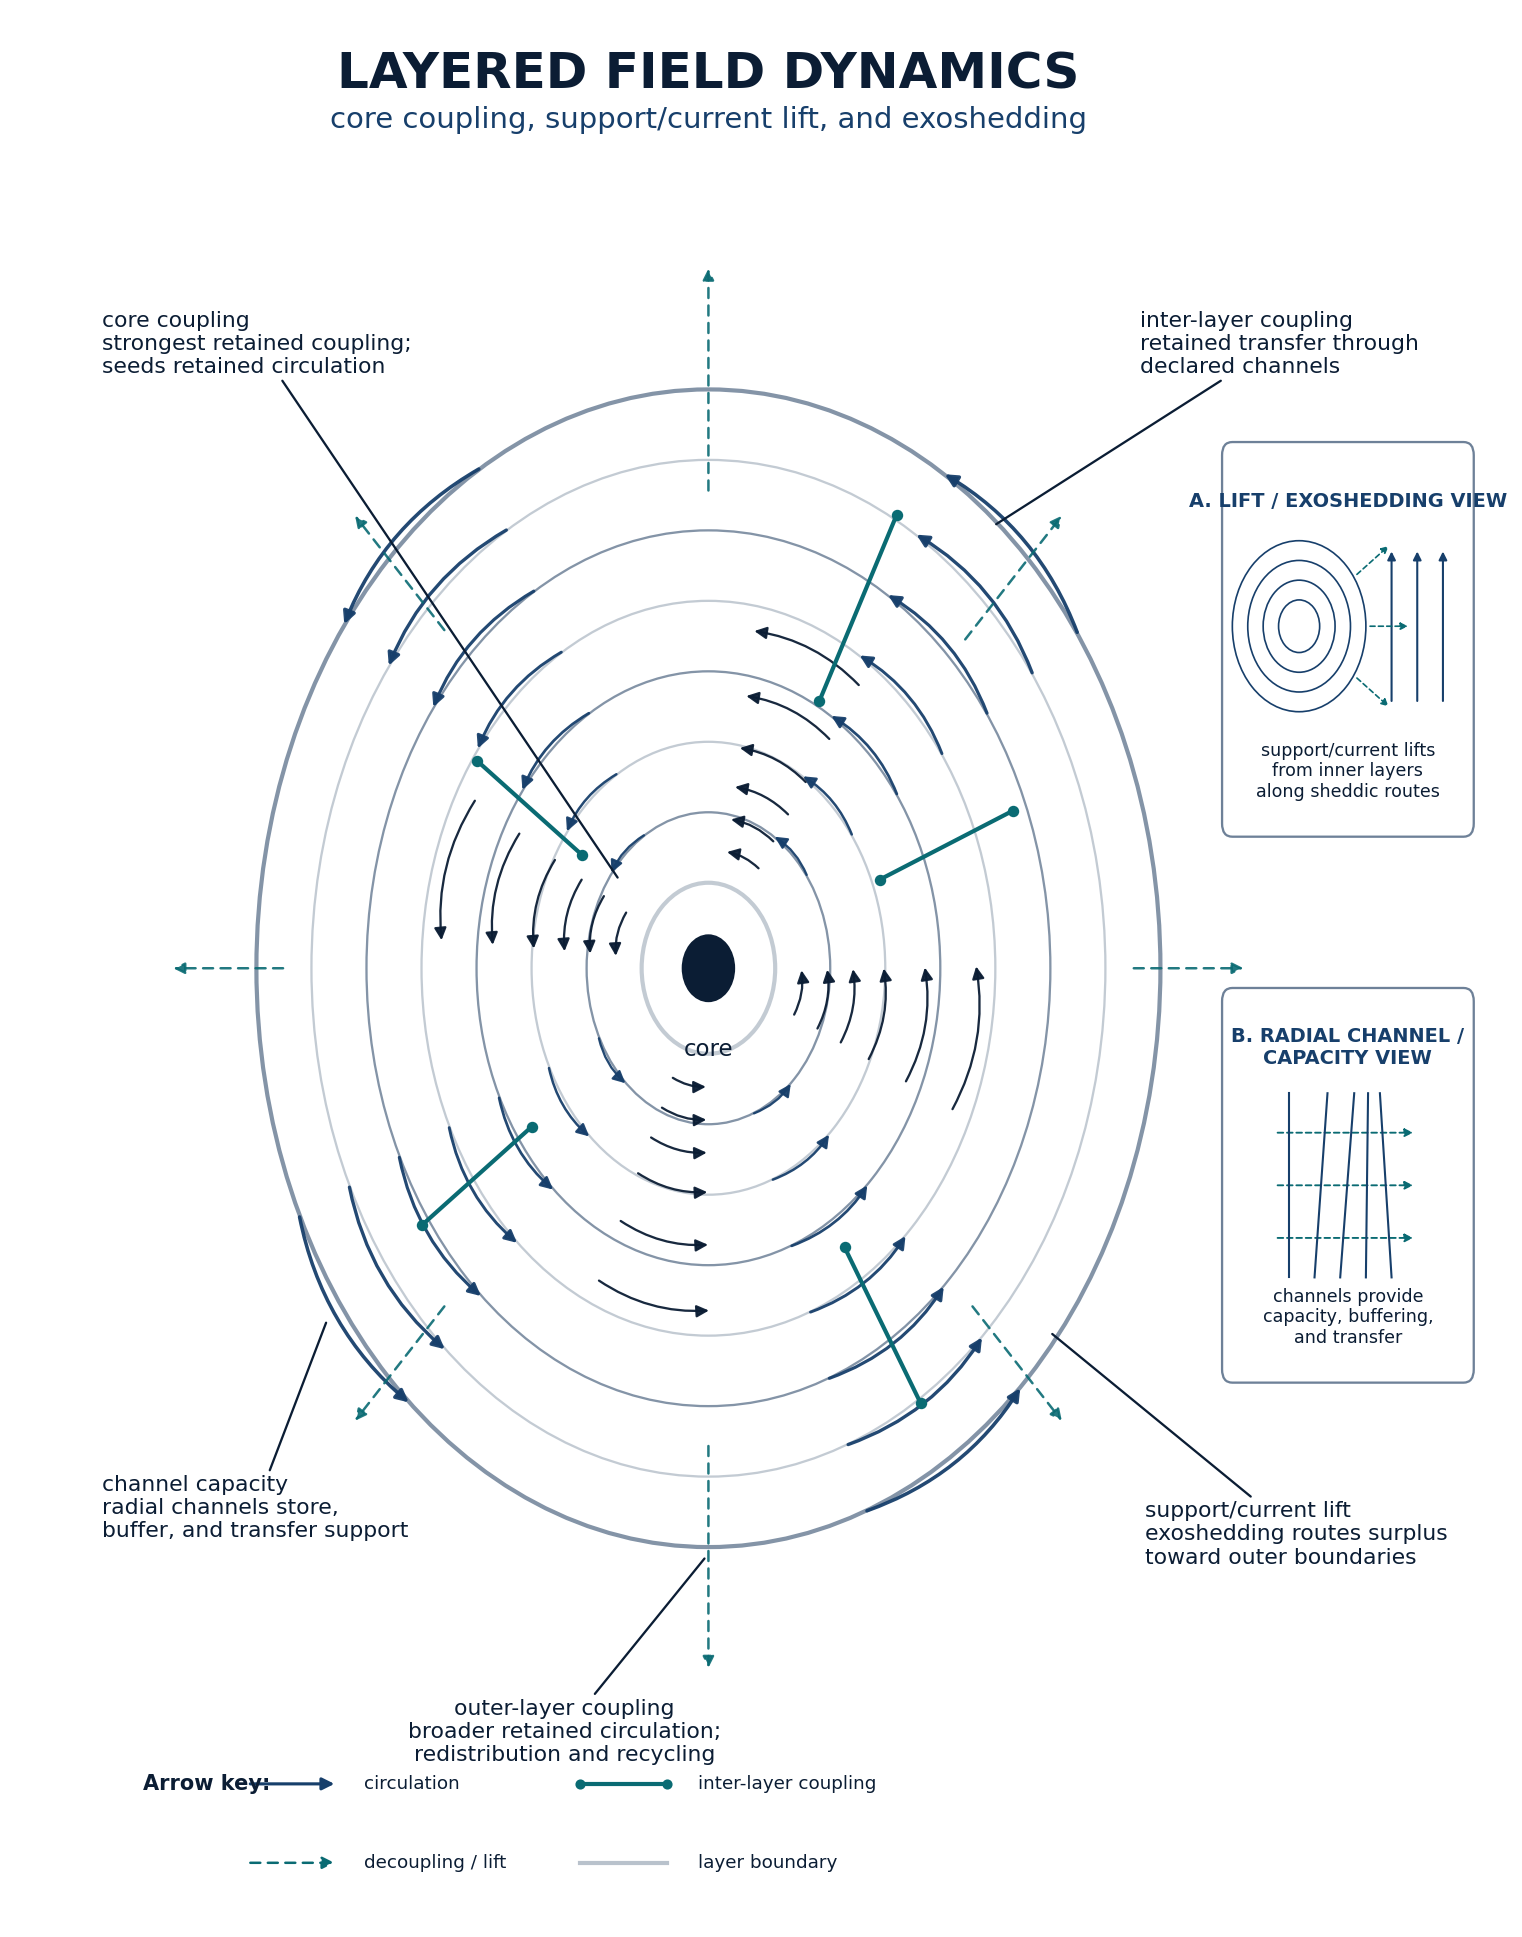
\includegraphics[width=0.82\linewidth]{figures_jpg/field_dynamics_layered.png}
\caption{Layered field dynamics. Boundaries separate layers; same-sense circulation remains on each layer; coupling arrows cross declared inter-layer channels; decoupling/lift arrows indicate exoshedding after closure surplus.}
\label{fig:field-dynamics-layered}
\end{figure}

\subsubsection{Finite SADAR moving-boundary dictionary}\label{subsec:finite-sadar-moving-boundary-dictionary}
For a moving boundary, the signed slice flux and window current remain
\[
\Phi^D_{\partial_T R_c}(t;B_c|t)
=
\sum_{e\in\partial_T R_c(t)}
\SADARop_{B_c|t}(C_e),
\]
\[
J^D_{\partial_T R_c}(\omega;B_c)
=
\sum_{t\in\omega}
\Phi^D_{\partial_T R_c}(t;B_c|t).
\]
The moving-boundary form is
\[
\Phi^D_{\partial_T R,\mathrm{mov}}(t)
=
\Phi^D_{\mathrm{cross}}(t)-\Phi^D_{\mathrm{sweep}}(t)+\Phi^D_{\mathrm{shedding}}(t).
\]
This is the finite SADAR moving-boundary dictionary. It is the boundary-current form of field dynamics. A nested moving field may carry bobbing as a signed sweep/shedding modulation on \(B_c|t\).

\subsection{Audit hooks}\label{sec:audit-hooks}
Audit hooks preserve structural checks.

\subsubsection{Spine audit}\label{subsec:spine-audit}
The audit passes when every retained occurrence at every finite depth has branch/hinge/branch incidence.

\subsubsection{Boundary audit}\label{subsec:boundary-audit}
The audit passes when slice flux and window current satisfy \(J^D_{\partial R}(\omega;B)=\sum_{t\in\omega}\Phi^D_{\partial R}(t;B|_t)\).

\subsubsection{SADAR audit}\label{subsec:sadar-audit}
Each returned-current channel has \(\ADAR_e=(A_e,D_e,R^{\mathrm{asym}}_e)\). The audit passes when the SADAR balance repeats over the declared returned-current channels on the inherited topology.

\subsubsection{Seat/enclosure routing audit}\label{subsec:support-enclosure-audit}
The audit passes when field-count scaling and seat-compatible shell/enclosure routing remain distinct calculations on the same declared boundary/window.

\subsubsection{Sheddic path audit}\label{subsec:sheddic-path-audit}
On a declared field and window, if \(X_{\mathrm{shedding}}(\partial F,\omega)>0\) and no sheddic path is declared through \(E_2\), \(\mathsf C_6\), \(\mathsf C_8\), \(\mathsf C_{10}\), or a higher even \(\mathsf C_{2n}\) form, the shedding statement fails on that scope. A sheddic path fails on the declared scope if its retained form violates the stated \(TTL_{\mathcal C}\) condition.



\subsubsection{Symbol audit}\label{subsec:symbol-audit}
SYM-A1. \(RD_B(C)\) is used only as reflection duration accessor.\\
SYM-A2. \(RCD\) is formed only through \(RD\bowtie_B R^{\mathrm{asym}}\).\\
SYM-A3. \(\rho^D=\operatorname{dur}(RCD)\) is declared before \(\rho^D_\omega\).\\
SYM-A4. \(\rho^D_\omega=\min(\rho^D,|\omega|)\) is the window-clipped duration participation.\\
SYM-A5. \(\delta_3\) records exact ternary signed residuals for internal integer fixtures.

\subsubsection{Cycle and polyrhythm audit}\label{subsec:cycle-polyrhythm-audit}
The cycle audit is certified when a retained field cycle is declared before any scalar duration accessor:
\[
\mathcal C_f[p{:}q]
\quad\text{before}\quad
RD\!\left(\mathcal C_f[p{:}q]\right).
\]
The polyrhythm audit is certified when each coupled cycle, its boundary/window, its reflection-duration accessor, and the coupling residual \(\Delta^{\mathrm{cyc}}_{ab}(B)\) are declared before the SADAR coupling term is formed.


\subsubsection{Fusion closure audit}\label{subsec:fusion-closure-audit}
The fusion closure audit passes when admitted curling-curl support forms, hinge \(\mu\), closure scope \(B\), branch/hinge/branch returned duration, and closure residual are declared before \(X_{\mathrm{shedding}}\) or any lifted support is formed. Chain reclosure is audited as iterated higher-scope fusion over admitted lifted supports. FRG-mediated reclosure is audited by the declared relation family and the computed identity \(T^\times=T^0+C^\times\).

\subsubsection{Fractal field ring-gate audit}\label{subsec:fractal-field-ring-gate-audit}
RG-A1. \(\mathfrak a\subset \mathcal A^{\mathrm{ret}}_8\) is declared.

RG-A2. \(B=(\partial_TF,\omega)\) is declared.

RG-A3. \((V_N,E_N)\) is declared.

RG-A4. \(\partial_T R_{\mathrm{ring}}\) is declared.

RG-A5. \(I\subseteq V_N\) and \(G=\{g_i:i\in I\}\) are declared.

RG-A6. \(\kappa_k\) is declared for every \(k\in K_{\mathrm{bin}}\).

RG-A7. \(E_{\mathrm{return}}\subseteq I\times I\) is declared.

RG-A8. Each path contribution uses \(\SADARop_{B|t}(C_\gamma)\) or declared \(\phi_\gamma(B|t)\).

RG-A9. \(\lambda_{\mathcal Y}:(T_k^\times)_k\mapsto\mathcal Y\) is declared as a value map.

RG-A10. \(T_k^\times-T_k^0=\sum C_{ij,k}^{\times}(B)\) is formed for declared exact integer fixtures.

RG-A11. Exact integer fixtures record \(\Delta^{\mathbb Z}\) and \(\delta_3\).

\subsubsection{Naming audit}\label{subsec:naming-audit}
A core name passes when it identifies a reusable relation pattern rather than a specific measured-sector carrier. Carrier names may appear in manual entries, comparison entries, benchmark entries, or quarantined external maps.

\subsubsection{AFC flux Stokes audit}\label{subsec:afc-flux-stokes-audit}
For a declared region \(R\) and scope \(B\), define
\begin{equation}
S_{\mathrm{int}}(R;B)
=
\sum_{i\in R}\sum_{j\in R}\phi_{ij}(B),
\label{eq:stokes-audit-internal}
\end{equation}
\begin{equation}
S_{\mathrm{div}}(R;B)
=
\sum_{i\in R}\operatorname{div}(i;B),
\qquad
S_{\partial}(R;B)
=
\sum_{\substack{i\in R\\j\notin R}}\phi_{ij}(B).
\label{eq:stokes-audit-sums}
\end{equation}
A valid declaration satisfies internal cancellation,
\begin{equation}
S_{\mathrm{int}}(R;B)=0,
\label{eq:stokes-audit-internal-zero}
\end{equation}
and boundary balance,
\begin{equation}
\mathcal E(R,B)
=
S_{\mathrm{div}}(R;B)-S_{\partial}(R;B)=0.
\label{eq:stokes-audit-residual}
\end{equation}
If \(S_{\mathrm{int}}(R;B)\ne0\), the declared orientation, sign, or antisymmetry fails on that scope. If \(\mathcal E(R,B)\ne0\), the declaration has a missing returned-current channel, incomplete boundary/window, undeclared sheddic path, or wrong channel content.

\subsubsection{Wave audit}\label{subsec:wave-audit}
A declared wave is recorded as cycle-carried distinction-information:
\[
Z_f=(\mathfrak c_f,I^c_f,B^e_f)
\to
Z_{f+1}=(\mathfrak c_{f+1},I^c_{f+1},B^e_{f+1}).
\]
Cycle compatibility carries wave continuity. Changed cycle compatibility routes excess burden into shedding, reclosure, pending return, or entropic duon current.
